\documentclass[a4paper]{report}
%\usepackage{afterpage}
\usepackage{amsmath}
\usepackage{amssymb}
\usepackage{caption}
\usepackage[mathscr]{eucal}
\usepackage{graphicx}
\usepackage{hyperref}
\usepackage{pgfplots}
\usepackage{subfigure}
\usepackage{xcolor}

% Uguaglianze/relazioni
\newcommand\aceq{\stackrel{\mathclap{\normalfont\mbox{ac}}}{\;=\;}}
\newcommand{\indep}{\mathrel{\text{\scalebox{1.07}{$\perp\mkern-10mu\perp$}}}}
\newcommand{\iidsim}{\stackrel{\text{iid}}{\sim}}
\newcommand{\indsim}{\stackrel{\indep}{\sim}}
\newcommand{\notindep}{\centernot{\indep}}

% Vari
\newcommand{\Ind}{\mathds{1}} % indicatrice
\newcommand{\im}{\operatorname{im}}
\newcommand{\markov}{\operatorname{Markov}}
\newcommand{\uu}[1]{\underline{#1}} % per i vettori
\newcommand{\IS}{È }
\renewcommand{\theta}{\vartheta} % è molto più bella

% Lettere fighe/corsive
\newcommand{\Ac}{\mathcal A}
\newcommand{\Bc}{\mathcal B}
\newcommand{\Cc}{\mathcal C}
\newcommand{\Dc}{\mathcal D}
\newcommand{\Ec}{\mathcal E}
\newcommand{\Fc}{\mathcal F}
\newcommand{\Gc}{\mathcal G}
\newcommand{\Hc}{\mathcal H}
\newcommand{\Ic}{\mathcal I}
\newcommand{\Jc}{\mathcal J}
\newcommand{\Kc}{\mathcal K}
\newcommand{\Lc}{\mathcal L}
\newcommand{\Mc}{\mathcal M}
\newcommand{\mm}{\mathscr m} %per la misura di Lebesgue
\newcommand{\Nc}{\mathcal N}
\newcommand{\Oc}{\mathcal O}
\newcommand{\Pc}{\mathcal P}
\newcommand{\Qc}{\mathcal Q}
\newcommand{\Rc}{\mathcal R}
\newcommand{\Sc}{\mathcal S}
\newcommand{\Tc}{\mathcal T}
\newcommand{\Uc}{\mathcal U}
\newcommand{\Vc}{\mathcal V}
\newcommand{\Wc}{\mathcal W}
\newcommand{\Xc}{\mathcal X}
\newcommand{\Yc}{\mathcal Y}
\newcommand{\Zc}{\mathcal Z}

% Doppia barra
\renewcommand{\AA}{\mathbb A}
\newcommand{\BB}{\mathbb B}
\newcommand{\CC}{\mathbb C}
\newcommand{\DD}{\mathbb D}
\newcommand{\EE}{\mathbb E}
\newcommand{\FF}{\mathbb F}
\newcommand{\GG}{\mathbb G}
\newcommand{\HH}{\mathbb H}
\newcommand{\II}{\mathbb I}
\newcommand{\JJ}{\mathbb J}
\newcommand{\KK}{\mathbb K}
\newcommand{\LL}{\mathbb L}
\newcommand{\MM}{\mathbb M}
\newcommand{\NN}{\mathbb N}
\newcommand{\OO}{\mathbb O}
\newcommand{\PP}{\mathbb P}
\newcommand{\QQ}{\mathbb Q}
\newcommand{\RR}{\mathbb R}
\renewcommand{\SS}{\mathbb S}
\newcommand{\TT}{\mathbb T}
\newcommand{\UU}{\mathbb U}
\newcommand{\VV}{\mathbb V}
\newcommand{\WW}{\mathbb W}
\newcommand{\XX}{\mathbb X}
\newcommand{\YY}{\mathbb Y}
\newcommand{\ZZ}{\mathbb Z}

% d nell'integrale
\newcommand{\de}{\mathrm d}
\newcommand{\dx}{\de x}
\newcommand{\dy}{\de y}
\newcommand{\dP}{\de P}
\newcommand{\dPP}{\de \PP}


\title{\texttt{bnplib}: A Nonparametric C++ Library}

\author{
Bruno Guindani \\
Elena Zazzetti \\
\\
Professor: Alessandra Guglielmi \\
Advisor: Mario Beraha \\
\\
\\
Politecnico di Milano \\
\\
}

\date{
TODO TODO, 2020
\\[250pt]
{\color{gray} {\url{https://github.com/poliprojects/BNPlib}}}
}

\begin{document}

\maketitle

\newpage\phantom{a}
%TODO fix page numbers



\thispagestyle{empty}
\begin{abstract}
We present a C++ library that exploits a Bayesian nonparametric setting in order to conduct unidimensional and multidimensional data analysis.
In such a setting, our main goals are density estimation and clustering analysis.
Several algorithms are available that make use of Gibbs sampling, building a Markov chain that reaches convergence at a reasonably fast pace.
In particular, we focused on implementing some algorithms introduced by Neal in 2000.
After running one of these algorithms, density and cluster estimation can then be conducted by using the provided auxiliary tools.
In this report, after an overview of the underlying Bayesian model and a roundup of the algorithms' state of the art, we delve into the details of our implementation and then present an example of data analysis, whilst providing the theoretical background for our estimates.
We also include a description for the implemented Python interface of this C++ library.
\end{abstract}
\setcounter{page}{4}

\tableofcontents

% Part 1
\part{Algorithms}

\chapter{Introduction}
This report presents the development of a C++ library containing Markov chain sampling algorithms for two major goals: estimation of the density and clustering analysis of a given set of data points.
In a Bayesian nonparametric setting, we focused on the Dirichlet process, one of the most widely used priors due to its flexibility and computational ease, and its extensions.
Hereafter, we will assume that the underlying model for the given data points is a Dirichlet process mixture model, which is an enhancement of the simpler Dirichlet model.
(For a more detailed discussion of the nonparametric models, as well as references for all theoretical details included in this section, see \cite{book} chapter 1 and 2.)


\section{A quick introduction to Bayesian statistics}
Bayesian statistics is a branch of mathematics with goals similar to regular statistics, which also holds the more accurate name of \emph{frequentist statistics}.
In both theories, data points $y$ are considered as realizations of random variables, often iid -- independent and identically distributed, with their distribution having one or more fixed and unknown parameters $\theta$, such as mean and variance in the Gaussian cases.
However, the frequentist approach is heavily focused on data and on pure information that can be extracted from it, for instance via estimates based on some form of sample mean.
By contrast, the Bayesian approach brings the data scientist's prior knowledge about the data into the picture; such knowledge is assumed to be approximately true, and the data is used to give it refinements and updates.
In a formal Bayesian setting, this prior knowledge takes on the form of a distribution $p(\theta)$ on the parameters of the data, called \emph{prior distribution}, or prior for short.
This is a crucial difference with respect to frequentist statistics, where parameters $\theta$ are unknown but assumed to be fixed, whilst in the Bayesian environment they are treated as \emph{random variables} for all intents and purposes.
This explains a major advantage of the Bayesian theory: it is naturally suited for non-pointwise estimates, mainly in the form of parameter distributions or their summary statistics, and therefore these are much easier to obtain than in the frequentist counterpart.
After taking the given data points into consideration, the parameter estimate provided by the prior is updated into the so-called \emph{posterior distribution} $p(\theta|y)$, or posterior for short, for the parameters.
The conditioning symbol indicates that the actual values of the realizations are used for a new better estimate of the parameters.
Similarly, since data are now distributed according to the random $\theta$, we use the notation $f(y|\theta)$ for the data distribution, which in this context is called \emph{likelihood}. \\
One can easily see that Bayesian statistics makes heavy use of conditional probabilities; so much so, in fact, that its very name is based off of the generalization of a well-known result for conditional probabilities, the \emph{Bayes theorem}.
In particular, this theorem states that, given $y_1, \dots, y_n$ iid random variables with joint likelihood $f(y|\theta) = f(y_1, \dots, y_n | \theta)$ and parameters with prior $p(\theta)$, the posterior for $\theta$ is given by
$$ p(\theta|y) = \frac{p(\theta) f(y|\theta)}{\int p(\theta) f(y|\theta) \, \dy} =
\frac{p(\theta) f(y|\theta)}{m(y)} \propto p(\theta) f(y|\theta).
$$
The denominator $m(y) = \int p(\theta) f(y|\theta) \, \dy$ is the \emph{marginal distribution} of data $y$, that is, its overall distribution without the knowledge of its parameters $\theta$.
It is often treated as an unimportant normalization constant, since it does not contain $\theta$, and therefore one often uses the last equality, which highlights the posterior's dependence on both the prior and the likelihood. \\
A coveted property for a Bayesian model is \emph{conjugacy}, that is to say that both the prior and the posterior distribution have the same form, e.g. they are both Gaussian distributions (most likely their parameters would both be different).
This property, or lack thereof, can make the difference between a posterior distribution being extremely easy to compute, and being flat out impossible to compute in closed form.
We shall see some examples of conjugate models later on in this section. \\
Finally, note that a Bayesian model may still employ frequentist tools to better incorporate data information into the prior; the most common example of this is setting the mean of the prior distribution as the sample mean of the given data.

\subsection{Advanced models} %TODO blargh
One is also allowed to use a more layered model, in which the parameters of the prior distribution, called \emph{hyperparameters}, also have prior distributions on them -- these are called \emph{hyperpriors}.
The result is as follows:
\begin{align*}
	y_1, \dots, y_n | \theta, \lambda &\iidsim f(y|\theta, \lambda) \\ %TODO can you remove lambda?
	\theta | \lambda &\sim p(\theta|\lambda) \\
	\lambda &\sim \Pi(\lambda)
\end{align*}
In fact, one can add as many layers as needed, adding priors to other priors' parameters, although one hyperprior like in the above model is generally considered enough to handle the complexity of most problems.
These are called \emph{hierarchical models}. \\
Another kind of advanced Bayesian structure is the so-called \emph{nonparametric model}, in which the entire likelihood is assumed to be random.
This means that there are infinitely many points which are randomly generated, that is, we have an infinite-dimensional parameter -- with a prior distribution for it, of course:
such a likelihood is an example of \emph{random probability measure}. \\
In the next pages, we will see some examples of elements composing these models, which can be divided into two classes: the \emph{mixture} component and the \emph{hierarchy} component.


\section{Dirichlet process model}
Let $M>0$, and let $G_0$ be a probability measure defined on the state space $S$.
A Dirichlet process with parameters $M$ and $G_0$, noted as $DP(M G_0)$, is a random probability measure $G$ defined on $S$ which assigns probability $G(B)$ to every set $B$ such that for each finite partition ${B_1,\dots,B_k}$ of $S$, the joint distribution of the  vector $(G(B_1),\dots,G(B_k))$ is the Dirichlet distribution with parameters $(MG_0(B_1),\dots,MG_0(B_k))$.\footnote{The Dirichlet distribution $\text{Dir}(\alpha_1, \dots, \alpha_k)$ is a $k$-dimensional generalization of the Bernoulli distribution, given parameters $\alpha_1,\dots,\alpha_k > 0$.
It has support in the $k-1$-dimensional simplex and its probability density function (p.d.f.) is
$$f(\textbf x) = \frac{1}{B(\alpha_1, \dots, \alpha_k)} \prod_{i=1}^k x_i^{\alpha_i-1}$$
with $B(\alpha_1, \dots, \alpha_k)$ being the $k$-dimensional Beta function that acts as a normalization constant.}
The value $M$ is called the \emph{total mass} or precision parameter, $G_0$ is the \emph{centering measure}, and the product $MG_0$ is the base measure of the DP. \\
Having observed the iid sample $\{y_1,\dots,y_n\} \subseteq \RR$, the basic DP model takes the following form:
\begin{equation}\label{dpm}
	\begin{aligned}
	y_i | G &\iidsim G, \quad i=1,\dots,n \\
	G &\sim DP(MG_0)
	\end{aligned}
\end{equation}
A key property is that the DP is conjugate with respect to iid sampling, so that the posterior base distribution is a weighted average of the prior base distribution $G_0$ and the empirical distribution of the data, with the weights controlled by $M$:
\begin{align}\label{dp-posterior}
	G | y_1,\dots,y_n \sim DP\left(M G_0 + \sum_{i=1}^n \delta_{y_i}\right).
\end{align}
Moreover, the marginal distribution for the data will be the product of the sequence of increasing conditionals:
\begin{align*}
	p(y_1,\dots,y_n)= p(y_1)\prod\limits_{i=2}^{n} p(y_i|y_1,\dots,y_{i-1}),
\end{align*}
with $y_1 \sim G_0$ and the conditional for $i=2,3,\dots$ being the following:
\begin{equation}
	\begin{aligned}
		p(y_i|y_1,\dots,y_{i-1}) =
		\frac{1}{M+i-1}\sum_{h=1}^{n-1} \delta_{y_h}(y_i) + \frac{M}{M+i-1} G_0(y_i).
	\end{aligned}
\end{equation}
The common pattern in both the above expression of the conditional and in the one for the posterior in (\ref{dp-posterior}) is that the centering measure $G_0$ is always given a weight proportional to $M$ (up to the normalizing constant $M+i-1$ in the former), whilst for the single points $y_i$, or the delta distribution centered in them, the weight is 1 for each datum, or $k$ if it has appeared $k$ times.
This is the heart of the so-called \emph{Polya's urn} representation model: the probability of a new value being equal to the ones before it is proportional to the number of times this value has appeared in the past, while the probability of the value being generated anew from $G_0$ is proportional to $M$.
Therefore, the more a value appears, the more likely it is for it to appear again in the future; instead, the total mass acts as the  ``cardinality'' of the action ``draw a new value''.
This is equivalent to having an urn which contains balls of different colors; each time a ball of a certain color is extracted, the ball is placed back into the urn alongside another new ball of the same color.
Furthermore, there's a chance proportional to $M$ that instead of extracting a ball from the urn, a ball of a random color, not necessarily one that is already present in the urn, is created and placed into the urn.
This urn will become relevant in the creation of the sampling algorithms implemented in this library. 
\\
Another important property is the discrete nature of the random probability measure $G$.
Because of this, we can always write $G$ as a weighted sum of point masses.
A useful consequence of this property is its stick-breaking representation, i.e. $G$ can be written as:
\begin{align*}
	G(\cdot) = \sum_{k=1}^{+\infty} w_k \delta_{m_k} (\cdot),
\end{align*}
with $m_k \iidsim G_0$ for $k\in\mathbb{N}$ and the random weights constructed as $w_k =v_k\prod\limits_{l<k} (1-v_l)$ where $v_k \iidsim Be(1,M)$. \\

One can replace the Dirichlet process in (\ref{dpm}) with any almost surely discrete random probability measure, for example a Pitman-Yor process (PY).
The PY process (see \cite{PY}, pp. 855-900) is a two-parameter extension of the Dirichlet process, parametrized by a discount parameter $0 \leq \alpha \leq 1$, a strength parameter $\theta > - \alpha$, and a base distribution $G_0$. 
Nevertheless, we will use the DP as our working example for the explanations in the next chapters. Developments are similar if another discrete process is used.

In many applications in which we are interested in a continuous density estimation, the discreteness can represent a limitation.
Oftentimes a Dirichlet process mixture (DPM) model is used, where the DP random measure is the mixing measure for the parameters of a parametric continuous kernel function.

\section{Dirichlet process mixture model}
Let $\Theta$ be a finite-dimensional parameter space and $G_0$ a probability measure on $\Theta$.
The Dirichlet process mixture (DPM) model convolves the densities $f(\cdot|\boldsymbol\theta)$ from a parametric family $\Fc = \{f(\cdot|\boldsymbol\theta), \boldsymbol\theta \in \Theta \}$ using the DP as mixture weights.
The obtained model has the following form:
\begin{equation}
	\begin{aligned}\label{dpm-1}
	y_i | G &\iidsim f_G(\cdot) = \int_\Theta f(\cdot|\boldsymbol\theta) \, G(\de\boldsymbol\theta), \quad i=1,\dots,n \\
	G &\sim DP(M G_0)
	\end{aligned}
\end{equation}
An equivalent hierarchical model is:
\begin{equation}
	\begin{aligned}\label{dpm-2}
	y_i | \boldsymbol\theta_i &\indsim f(\cdot|\boldsymbol\theta_i), \quad i=1,\dots,n \\
	\boldsymbol\theta_i | G &\iidsim G, \quad i=1,\dots,n \\ 
	G &\sim DP(M G_0)
	\end{aligned}
\end{equation}
where the \emph{latent variables} $\boldsymbol\theta_i$ are introduced, one per unit.
Since $G$ is discrete, we know that two independent draws $\boldsymbol\theta_i$ and $\boldsymbol\theta_j$ from $G$ can be equal with positive probability.
In this way the DPM model induces a probability model on clusters of $\boldsymbol\theta_i$.
An object of interest that derives from this model is the partitioning induced by the clustering. \\%, as well as the density estimation. \\
Considering $n$ data points, each $\boldsymbol\theta_i$ will have one of the $k$ unique values $\boldsymbol\phi_{j}$.
An estimation of the number of the unique values is $M\log(n) \ll n$.
Defining  $\boldsymbol c= (c_1,\dots,c_n)$ the \emph{allocation} parameters to the clusters such that $c_i = j$ if $\boldsymbol\theta_i = \boldsymbol\phi_j$, model (\ref{dpm-2}) can be thought of as the limit as $K \to +\infty$  of a finite mixture model with $K$ components (recall instead that $k$ is the number of unique values):
\begin{equation}
	\begin{aligned}\label{dpm-disc}
		y_{i}|\boldsymbol{\phi}_1,\dots,\boldsymbol{\phi}_k,c_{i} &\indsim f(\cdot|\boldsymbol\phi_{c_{i}}), \quad i=1,\dots,n \\
		c_{i}|\mathit{\mathbf{p}}&\iidsim \sum_{j=1}^K\mathit{p_j} \delta_j(\cdot), \quad i=1,\dots,n \\
		\boldsymbol\phi_{c} & \iidsim G_{0}, \quad c=1,\dots,k \\
		\mathbf{p} &\sim \operatorname{Dir}(M/K,\dots,M/K)
	\end{aligned}
\end{equation}
where $\mathbf{p}=(p_1,\dots,p_K)$ represents the mixing proportions for the clusters and each $\boldsymbol\theta_i$ is characterized by the latent cluster $c_i$ and the corresponding parameters $\boldsymbol\phi_{c_i}$.

\section{Normal Normal-InverseGamma hierarchy} \label{nnig}
A very common choice for the DPM model (\ref{dpm-1}) is the Normal Normal-InverseGamma (NNIG) hierarchy, opting for a Normal kernel and the conjugate Normal-InverseGamma as base measure $G_0$.
The InverseGamma is the distribution of a random variable $Y$ such that $Y^{-1}$ follows a Gamma distribution
\footnote{The Gamma distribution $\text{Gamma}(\alpha,\beta)$ has parameters $\alpha,\beta > 0$, and has support over all positive values, which is ideal for variances or their inverse, the precision.
Its p.d.f. is
$$f(x) = \frac{\beta^\alpha}{\Gamma(\alpha)} x^{\alpha-1} \exp\{-\beta x\}$$
with $\Gamma(\alpha)$ being the Euler-Gamma function.}.
That is, letting $\boldsymbol\theta=(\mu,\sigma)$, we have:
\begin{equation}
	\begin{aligned}
		f(y|\boldsymbol\theta)&=N(y| \mu ,\sigma^2),  \\
		G_0(\boldsymbol\theta|\mu_0,\lambda_0, \alpha_0, 	\beta_0)
		&=N\left(\mu | \mu_0 ,\frac{\sigma^2} {\lambda_0}\right) \times \text{Inv-Gamma}(\sigma^2|\alpha_0, \beta_0 ).
	\end{aligned}
\end{equation}
Note that in this model we have a full prior for $\sigma^2$ and instead a prior for $\mu$ that is conditioned on the value of $\sigma^2$.
Thanks to conjugacy, the predictive distribution for a new observation $\widetilde{y}$ (which coincides with the marginal distribution for a known datum) can be computed analytically, finding a Student's $t$ (see \cite{integral} section 3.5):
\begin{align*}
	p(\widetilde{y}|\mu_0,\lambda_0, \alpha_0, \beta_0) =
	\int_\Theta f(\widetilde{y}|\boldsymbol\theta) \, G_0(\de\boldsymbol\theta) =
	t_{\widetilde \nu}\left(\widetilde{y}|\widetilde{\mu},\widetilde{\sigma}^2\right)
\end{align*}
where the following parameters are set:
$$
	\widetilde{\nu}=2 \alpha_0, \quad
	\widetilde{\mu}=\mu_0, \quad
	\widetilde{\sigma}^2= \frac{\beta_0(\lambda_0+1)}{\alpha_0 \lambda_0}
$$
We highlight the definition of the Student's $t$ distribution in the general multivariate case, since it will often come up in calculations.
Given the degrees of freedom $\nu > 0$, the $k$-dimensional location vector $\boldsymbol\mu$, and the $k$-by-$k$, positive semi-definite scale matrix $\Sigma$,
the $k$-dimensional Student's $t$ distribution $t_\nu(\boldsymbol\mu, \Sigma)$ has the following p.d.f.:
$$ f(\textbf x) = \frac{\Gamma\left(\frac{\nu+k}{2}\right)}{\Gamma(\nu/2) \sqrt{(\nu\pi)^k \det(\Sigma)}} \left( 
1+\frac{1}{\nu}(\textbf x - \boldsymbol \mu)^T\Sigma^{-1}(\textbf x - \boldsymbol \mu) \right)^{-(\nu+k)/2}.
$$
In the univariate case, the scale parameter is written as $\sigma^2$.
When no location and scale are provided, it is understood that the symbol $t_\nu$ refers to the one-dimensional case with standard parameters, that is $\mu=0$ and $\sigma^2 = 1$. \\
Going back to the NNIG hierarchy, the posterior distribution is again a Normal-InverseGamma (see \cite{integral} section 3.3) thanks to conjugacy:
\begin{align*}
	p(\boldsymbol\theta|y_1,\dots,y_n,\mu_0,\lambda_0, \alpha_0, \beta_0)=N\left(\mu | \mu_n ,\frac{\sigma^2} {\lambda_n}\right) \times \text{Inv-Gamma}(\sigma^2|\alpha_n, \beta_n )
\end{align*}
with $\bar{y}$ indicating the sample mean of the data and:
\begin{gather*}
\mu_n=\frac{\lambda_0 \mu_0 \bar{y} + n}{\lambda_0 + n}, \qquad \lambda_n = \lambda_0 + n, \qquad
\alpha_n = \alpha_0 + \frac{n}{2}, \\
\beta_n= \beta_0 + \frac{1}{2}\sum_{i=1}^{n} (y_i-\bar{y})^2 + \frac{\lambda_0 n(\bar{y}-\mu_0)^2}{2(\lambda_0 + n)}.
\end{gather*}


\section{Normal Normal-Wishart hierarchy} \label{nnw}
The multivariate extension of the above hierarchy is the Normal Normal-Wishart (NNW) model:
\begin{equation}
	\begin{aligned}
		f(\textbf y|\boldsymbol\theta) &= N(\textbf y | \boldsymbol\mu ,T^{-1}), \\
		G_0(\boldsymbol\theta|\boldsymbol \mu_0, \lambda, T_0, \nu)
		&= N\left(\mu | \boldsymbol\mu_0, (\lambda T)^{-1}\right) \times \text{Wish}(T|T_0, \nu).
	\end{aligned}
\end{equation}
In this case $\boldsymbol\theta=(\boldsymbol\mu, T)$ and $\textbf y \in \RR^k$.
Note that the scale is parametrized in a different way compared to univariate case, with the second unique value being the precision matrix $T = \Sigma^{-1}$, the inverse of the covariance matrix.
As such, the Wishart distribution\footnote{The Wishart distribution $\text{Wish}(T_0, \nu)$ is a $k$-dimensional generalization of the Gamma distribution.
It has support over all matrices $X \in \RR^{k \times k}$ that are positive semi-definite.
Its p.d.f. is
$$f(X) = \frac{ (\det(X))^{(\nu-k-1)/2} \, \exp\{-\frac{1}{2} \text{tr}(T_0^{-1} X)\} }{ 2^{\nu k/2} \, (\det(X))^{\nu/2} \, \Gamma_k(\nu/2) } $$
with $\Gamma_k(\alpha)$ being the $k$-dimensional Gamma function.} is used instead of its inverse counterpart. \\
This hierarchy has similar properties to the NNIG case, namely conjugacy and a marginal distribution with the form of a multivariate Student's $t$. \\
The marginal is:
$$ p(\widetilde{\textbf y} | \boldsymbol\mu_0, \lambda, T_0, \nu) = t_{\widetilde\nu} (\widetilde{\textbf y} | \widetilde{\boldsymbol\mu}, \widetilde\Sigma) \qquad
$$
with:
$$ \widetilde{\nu} = 2\nu - k + 1, \qquad \widetilde{\boldsymbol{\mu}} = \boldsymbol{\mu}_0, \qquad
\widetilde{\Sigma} = T_0^{-1} \left(\nu - \frac{k-1}{2}\right) \frac{\lambda}{\lambda+1}
$$
while the posterior distribution is:
\begin{align*}
p(\boldsymbol\theta|\textbf y_1,\dots,\textbf y_n,\boldsymbol\mu_0,\lambda, T_0, \nu)=N\left(\boldsymbol\mu | \boldsymbol\mu_n, \frac{1}{\lambda_n}\Sigma\right) \times \text{Wish}(\Sigma|T_n, \nu_n)
\end{align*}
with  (again, $\bar{\textbf y}$ is the sample mean):
\begin{gather*}
\boldsymbol\mu_n = \frac{1}{\lambda+n} (\lambda\boldsymbol \mu_0 + n \bar{\textbf y}), \qquad \lambda_n = \lambda + n, \qquad \nu_n = \nu + \frac{n}{2}, \\
T_n = T_0^{-1} + \frac{1}{2}\sum_{i=1}^{n} (\textbf y_i-\bar{\textbf y})(\textbf y_i-\bar{\textbf y})^T + \frac{\lambda n}{2(\lambda + n)}(\bar{\textbf y}-\boldsymbol\mu_0)(\bar{\textbf y}-\boldsymbol\mu_0)^T.
\end{gather*}

\chapter{Algorithms} \label{algo}
For the task of density estimation, we investigated several Markov chain methods to sample from the posterior distribution of a DPM model. \\
Starting from the hierarchical model (\ref{dpm-1}), a first direct approach is simply drawing values for each $\boldsymbol\theta_i$ from its conditional distribution, given the data and the other $\boldsymbol\theta_j$.
However, as previously discussed, we have high probability for ties among them which can lead to slow convergence, since the $\boldsymbol\theta_i$ are not updated for more than one observation simultaneously. \\
For this reason, special attention was paid to the three methods we present in this chapter.
They are Gibbs samplers with a similar base structure, sharing the two steps for the sampling of the allocations $\mathbf{c}$ and of the unique values $\boldsymbol\phi_c$.
The set of allocations and unique values at a given iteration constitutes the \emph{state} of that iteration.
As the state is being updated at each iteration, a \emph{chain} is formed and the mean of the state values eventually reaches convergence, as well as the estimate for the data distribution, as we will see in section \ref{dens-estim}.
Moreover, all methods can be extended with additional steps for hierarchical extensions.
For example, we can place priors to hyperparameters of the centering measure $G_0$ or to the total mass $M$.

\section{Neal's Algorithm 2} \label{neal2}
In order to speed up convergence in case of ties, Neal first proposed (see \cite{neal} section 3 as well as \cite{book} chapter 2) a more efficient Gibbs sampling method based on the discrete model (\ref{dpm-disc}), but where the mixing proportions $\textbf{p}$ have been integrated out.
We will refer to this method as Neal's Algorithm 2, or \verb|Neal2| for short.
Before getting to the algorithm, let us start from the discrete model (\ref{dpm-disc}).
Assuming that the current state of Markov chain is composed of $(c_1,\dots,c_n)$  and the unique values $\boldsymbol\phi_c$ for all $c=1,\dots,k$, the Gibbs sampler should first draw a new value $c$ for each $c_i$ according to the following probabilities:
\begin{align}
	\hspace{-25pt}
	\vspace{-12pt}
	\text{If $c=c_j$ for some $j$: }
	\PP(c_{i}=c | \boldsymbol c_{-i}, y_{i},\boldsymbol{\phi}_1,\dots,\boldsymbol{\phi}_k) \propto \frac{n_{-i,c} + M/{K}}{n-1+M} f(y_{i}|\boldsymbol\phi_{c}) 
\end{align}
where $\boldsymbol c_{-i}$ is $\boldsymbol c$ minus the $i$-th component, and $n_{-i,c}$ is the number of $c_j$ equal to $c$ excluding $c_i$.
The transition to the infinite case, that is, to the reference DPM model (\ref{dpm-2}), is handled by taking the limit as $K$ goes to infinity in the conditional distribution of $c_i$, which becomes as follows:
\begin{equation}
	\begin{aligned} \label{probasneal2}
	\hspace{-25pt}
	\vspace{-12pt}
	\text{If $c=c_j$ for some $j$: }
	\PP(c_{i}=c | \boldsymbol c_{-i}, y_{i}, \boldsymbol{\phi}_1,\dots,\boldsymbol{\phi}_k) &\propto \frac{n_{-i,c} }{n-1+M} f(y_{i}|\boldsymbol\phi_{c}) \\
	\PP(c_{i}\neq c_{j} \text{ for all } j | \boldsymbol c_{-i}, y_{i}, \boldsymbol{\phi}_1,\dots,\boldsymbol{\phi}_k) &\propto \frac{M }{n-1+M} \int_{\Theta} f(y_{i}|\boldsymbol\theta) \, G_0(\de\boldsymbol\theta)
	\end{aligned}
\end{equation}
and considering only the $\boldsymbol\phi_c$ associated with some observation, keeping the sampling finite and thus computationally feasible.
The former expression is proportional to the cardinality of that cluster (excluding the $i$-th observation), while the latter is instead proportional to the total mass $M$ and represents the probability of creating a new cluster.
Moreover, the integral $m(y_i) = \int_{\Theta} f(y_{i}|\boldsymbol\theta) \, G_0(\de\boldsymbol\theta)$ represents the \emph{marginal distribution} of the data points evaluated in $y_i$. \\
Let us now introduce the actual \verb|Neal2| algorithm, which works iteratively in two steps, in which we sample $(\boldsymbol{c}_1,\dots,\boldsymbol{c}_n)$ and $(\boldsymbol{\phi}_1,\dots,\boldsymbol{\phi}_k)$, respectively.
First, for each observation $i$, $c_i$ is updated according to the conditional probabilities (\ref{probasneal2}).
It can be set either to one of the other components currently associated with some observation, or to a new mixture component.
If the new value of $c_i$ is different from all the other $c_j$, a value for $\boldsymbol\phi_{c_i}$ is created by drawing it from the posterior distribution $H_i$, given the prior $G_0$ and the single observation $y_i$; this means that in this case, a new cluster has been created. \\
Then, for all clusters, the sampling of their unique value $\boldsymbol\phi_c$ is conducted by considering their posterior distribution given the prior $G_0$ and all observations belonging to that cluster.
The probability of setting $c_i$ to a new component involves the computation of the marginal, which is difficult to compute in the non-conjugate case, as well as the sampling from the posterior $H_i$.
For this reason, the algorithm is only used under conjugacy and hence it is possible to exactly compute the integral.

\section{Neal's Algorithm 8} \label{neal8}
To handle non-conjugate priors, Neal proposed (see \cite{neal} section 6 and \cite{book} chapter 2) a second Markov chain sampling procedure, the \verb|Neal8| algorithm, where the state is extended by the addition of $m$ auxiliary parameters.
This technique allows to update the $c_i$ while avoiding the integration with respect to $G_0$ for the computation of the marginal. \\
In this case the sampling probabilities for the $c_i$ given all other $c_j$ are:
\begin{equation}
	\begin{aligned}
		\hspace{-25pt}
		\vspace{-12pt}
		\text{If $c=c_j$ for some $j$: } \PP(c_i=c | \boldsymbol c_{-i}) &= \frac{n_{-i,c}}{n-1+M}   \\
		\PP(c_{i}\neq c_{j} \text{ for all } j) &=\frac{M }{n-1+M}
	\end{aligned}	
\end{equation}
where the latter probability of creating a new cluster is evenly split among the $m$ auxiliary components, which will also be referred to as the \emph{auxiliary blocks}.
Maintaining the same structure as the \verb|Neal2| algorithm, \verb|Neal8| is composed of two steps, where the components of the Markov chain state $(\boldsymbol{c}_1,\dots,\boldsymbol{c}_n)$ and $(\boldsymbol{\phi}_1,\dots,\boldsymbol{\phi}_k)$ are repeatedly sampled.
\begin{figure}[h]
    \centering
    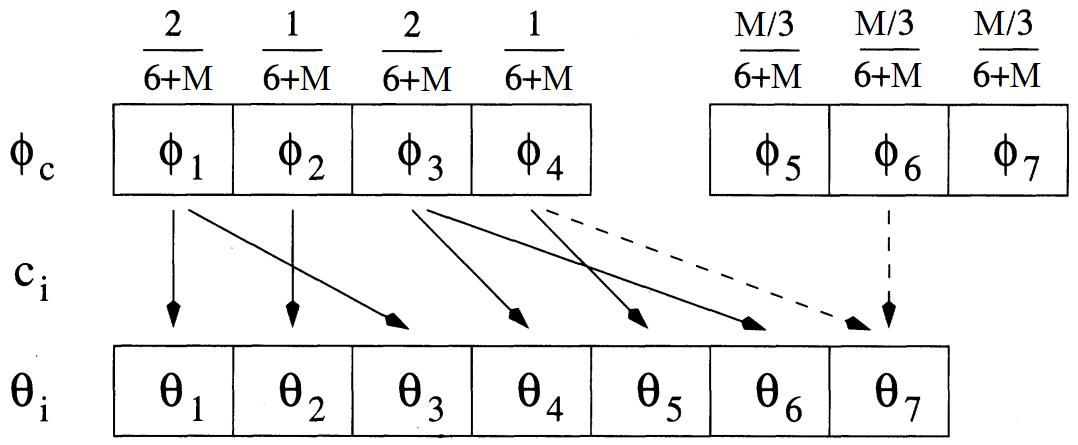
\includegraphics[width=0.9\textwidth]{etc/neal8.png}
    \captionsetup{labelformat=empty}
    \caption{Graphical representation of the variables: the allocations are visualized as arrows linking each $\boldsymbol\theta_i$ with either one of the four old clusters or one of the new components (image taken from \cite{neal})}
    \label{fig:neal8}
\end{figure}

The first step scans all the observations and evaluates each $c_i$.
If it is equal to some other $c_j$, i.e. if the current cluster of observation $i$ is not a singleton, then all auxiliary variables are iid drawn from $G_0$.
If instead the cluster corresponding to $c_i$ is a singleton, then it is linked to one of the auxiliary blocks (i.e. the first one, without loss of generality) while keeping its old unique value $\boldsymbol\phi_{c_i}$ (as shown in the above figure), whereas the other blocks are drawn normally from $G_0$ as before.
Then, $c_i$ is updated according to the following conditional probabilities:
\begin{equation}
	\begin{aligned} \label{neal8prob}
		\PP(c_{i}=c | \boldsymbol c_{-i}, y_{i}, \boldsymbol\phi_{1},\dots,\boldsymbol\phi_{h}) \propto
		\begin{cases}
			\dfrac{n_{-i,c}}{n-1+M}f(y_{i}|\boldsymbol\phi_{c}), & \mbox{for } 1 \leq c \leq k^{-} \\
			\\
			\dfrac{M/m}{n-1+M}f(y_{i}|\boldsymbol\phi_{c}), & \mbox{for } k^{-}+1 < c \leq h,
		\end{cases}
	\end{aligned}
\end{equation}
indicating with $k^{-}$ the number of distinct $c_j$ excluding the current $c_i$ and setting $h=k^{-}+m$.
Again, the probabilities of being placed in an already existing cluster or in a newly created cluster are proportional to the cluster's cardinality (sans observation $i$) and to the total mass, respectively. \\
Once all the $\boldsymbol\phi_c$ that are no longer associated with any observation are discarded, the algorithm proceeds, for each cluster, with the sampling of $\boldsymbol\phi_c$ from the posterior computed with the observations of the specific cluster, similarly to the \verb|Neal2| algorithm.

\section{Blocked Gibbs}
Another Gibbs sampling method that is applicable in the considered DPM model is the one proposed by Ishwaran and James (see \cite{james} section 5), where the prior $P$ is assumed to be a finite dimensional stick-breaking measure, allowing the update of whole blocks of parameters.
A key point of the method is that it does not marginalize over the prior; instead, by grouping more variables together, it samples from their joint distribution conditioned on all other variables.
This sampler needs to draw from the following conditionals:
\begin{align}
	\boldsymbol\phi_1,\dots,\boldsymbol\phi_k &\sim \Lc(\cdot | c_1,\dots,c_n, \boldsymbol{y}) \nonumber \\
	c_1,\dots,c_n &\sim \Lc (\cdot | \boldsymbol\phi_1,\dots,\boldsymbol\phi_k,\boldsymbol{p}, \boldsymbol{y}) \nonumber \\
	\boldsymbol{p} &\sim \Lc (\cdot | c_1,\dots,c_n) \nonumber
\end{align}
The drawing of the unique values can also be handled in the non-conjugate case by applying standard Markov chain Monte Carlo methods. \\
This algorithm is not explored in detail as it has not implemented yet in our library.
For a full explanation, see \cite{james}.

\chapter{Estimates} \label{chap-esimates-1}
We recall that the aim of these chain-producing algorithms is to build estimates for both the actual clustering structure of the data and its probability distribution, i.e. their likelihood.
We shall now explain how we achieve such estimates.
Note that these will be identical regardless of the dimension of the data points.


\section{Cluster estimation}
Suppose we wish to estimate the real clustering of the data, assuming the DPM model holds true.
Since the proposed algorithms repeat the same steps for many iterations, they will run through just as many states, i.e. combinations of unique values and clusters, which represent a clustering structure.
Therefore, one might think that a first rough estimate for the real clustering could be the \emph{final clustering}, that is, the state values corresponding to the last iteration of the algorithm.
However, due to the oscillating behavior of the clusters (as we shall show later on by performing tests), the last clustering is far from being guaranteed to be the optimal one.
Instead, we chose to implement a \emph{least square} estimate.
More specifically, we examine the state values provided by each iteration, then we select the one that minimizes the squared posterior \emph{Binder's loss function}, which gives cost 0 to a pair of points which are correctly assessed to be in the same cluster, and cost 1 to a pair of points which are placed in the same cluster but are actually in different ones.
An equivalent approach (see \cite{beep-bayes} lecture on BNP clustering) is computing the so-called \emph{dissimilarity matrix} for each iteration, computing its sample mean over all iterations, and finding the iteration that is the closest to the mean with respect to the \emph{Frobenius norm}, which the sum of squares of the matrix entries. 
More specifically, for each iteration $k$, the dissimilarity matrix $D^{(k)}$ is a symmetric, binary $n$-by-$n$ matrix (where $n$ is the number of available observations) whose entries $D^{(k)}_{ij}$ are $1$ if datum $i$ and $j$ are placed in the same cluster at iteration $k$ and $0$ otherwise.
After each $D^{(k)}$ and the sample mean $\bar{D} = \frac{1}{K} \sum_k D^{(k)}$ are computed, where $K$ is the number of iterations (not counting the ones in the burn-in phase), the best clustering $\hat{k}$ is found by minimizing the Frobenius norm of the difference with $\bar{D}$:
$$
\hat{k} = \argmin_k \left\lVert D^{(k)} - \bar D \right\rVert_F^2 = \argmin_k \sum_{i,j} \left( D^{(k)}_{ij} - \bar{D}_{ij} \right)^2.
$$
Note that by virtue of the involved matrices being symmetric, the minimization of the latter summation is equivalent to the one computed only for those entries $(i,j)$ such that $i<j$.
One can prove that the described algorithms \emph{converge in mean}, but not in the single iterations.
That is, the last iterations of the algorithm have no higher probability than the first ones of being the ``best'' cluster estimate; in fact, the algorithm has quite the \emph{oscillating behavior} in its single-iteration estimates, starting with the number of clusters at each iteration, as we will see in the last part of the report.
Instead, it is the mean of all dissimilarity matrices that converges to the ``best'' clustering structure: the more iterations are run, the better the approximation provided by the mean becomes.
(The number of iterations required is actually surprisingly small: we will show that even a few hundreds are enough to get a good estimate.)
Since the mean itself is obviously not a valid dissimilarity, as it is not binary-valued, we choose the one valid iteration matrix that best approximates it.
This guarantees the correctness of this least square estimate, at it is the closest available approximation to the mean dissimilarity matrix.



\section{Density estimation}\label{dens-estim}
The other important application of iterative BNP algorithms is the estimation of the density according to which the data points are distributed.
This is done slightly differently in both the \verb|Neal2| and \verb|Neal8| algorithms, as the former can exploit the conjugacy of the hierarchical model.
Just like for the cluster estimate, the computation will need to access all iterations run by the algorithm.
In either algorithm, suppose that iteration $k$ has $J$ clusters, that is, $j=0:J-1$.
Given a point $y$, we compute the local estimate of the density, which is built only taking iteration $k$ into account:
\begin{equation}\label{localdens}
	\begin{aligned}
		\hat f^{(k)}(y) \ = \ \sum_j \frac{n^{(k)}_j}{M+n} f\left(y | \boldsymbol{\phi}^{(k)}_j\right) \ + \ \frac{M}{M+n} m(y)
	\end{aligned}
\end{equation}
where $n^{(k)}_j$ is the cardinality of cluster $j$.
That is, the local estimate is a weighted mean of the likelihood given the unique values $\boldsymbol{\phi}^{(k)}_j$ of cluster $j$ and the marginal distribution $m(y)$ computed in the point.
Again, note that the relative weights of the clusters are proportional to their size $n^{(k)}_j$, while the ``virtual'' cluster of the marginal counts as having size $M$, the total mass parameter ($n$ is the total number of observations, as per usual).
The marginal distribution is only known under the conjugacy assumption in the \verb|Neal2| algorithm.
In particular, for both an NNIG and an NNW model $m(y)$ is a Student's $t$ as explained in section \ref{nnig} onwards.
In the \verb|Neal8| algorithm, $m(y)$ is not available in closed form, and thus it is replaced in the above formula by the following approximation:
\begin{equation}\label{margneal8}
	\begin{aligned}
		\hat m(y) = \frac{1}{m} \sum_{h=0}^{m-1}  f\left(y | \boldsymbol{\phi}_h\right)
	\end{aligned}
\end{equation}
where we use $m$ unique values, that is, one for each of the $m$ auxiliary blocks of the algorithm, drawn from the base measure: $\boldsymbol{\phi}_{h} \overset{\text{iid}}{\sim} G_0, \ h=0:m-1$. \\
Finally, the total \emph{empirical density} is computed as the mean over all $K$ iterations:
$$
\hat f(y) = \frac{1}{K} \sum_k \hat f^{(k)}(y).
$$
Again, this estimate approaches the true posterior density of the data thanks to the convergence in mean of the chain.


% Part 2
\part{Implementation}

\chapter{Hierarchy classes}
First of all, we must describe the auxiliary classes that are used as parameters for the algorithms:
\begin{itemize}
	\item The \verb|BaseMixture| class, contain all information about the mixing part of the BNP algorithm, namely the way of weighing the insertion of data in old clusters vs the creation of new clusters. The class has methods that provide mass probabilities for the two aforementioned events. We implemented the \verb|BaseMixture| class as an abstract class, and two derived classes: the \verb|DirichletMixture| and the \verb|PitYorMixture|. The derived classes have its own parameters and could be extended by adding prior distributions on these.

	\item The \verb|Hypers| classes contain all information about the hyperparameters of the hierarchy, including their values (if fixed) or their prior distributions (if not). We implemented the \verb|HypersFixedNNIG| class, which contains fixed hyperparameters for an NNIG hierarchy, and the \verb|HypersFixedNNW| class for an NNW hierarchy. Both classes provide setters and getters for parameters with validity checks for the inserted values.
	
	\item The \verb|HierarchyBase<Hypers>| class is an abstract template class that accept any \verb|Hypers| class as template parameter.
	
	
This template class represents a hierarchy object in a generic iterative BNP
algorithm, that is, a single set of unique values with their own prior
distribution attached to it. These values are part of the Markov chain's
state chain which develops as the iterations of the algorithm increase, updating them providing the data related to the specific hierarchy and their prior distribution.
They are simply referred to as the state of the hierarchy. 

The class stores the current unique values in the protected member \verb|state|, a vector of parameter matrices.
Since the prior distribution for the state is often the same across multiple
different hierarchies, the hyperparameters object is accessed via a shared
pointer, stored as protected member, and this is why \verb|Hypers| is required as a template parameter for the class. 

	A \verb|BaseHierarchy<Hypers>| class also contains methods to:
	\begin{itemize}
		\item evaluate the marginal distribution (provided it is known in closed form) and the log-likelihood in a given set of points, given the current \verb|state|;
		\item compute the posterior parameters with respect to a given set of observations;
		\item generate new values for the \verb|state| both according to its prior and to its posterior distribution;
		\item get and set class members, as with the other classes.
	\end{itemize}


The hierarchy classes we implemented that inherits from this class are the \verb|HierarchyNNIG| class, which represents the Normal Normal-InverseGamma hierarchy for univariate data, and the \verb|HierarchyNNW| class, which represents the Normal Normal-Wishart hierarchy for multivariate data.

In particular the \verb|state| in the \verb|HierarchyNNIG| class holds the values for $\boldsymbol\phi = (\mu,\sigma)$, i.e.  location and scale, while the \verb|HierarchyNNW| class stores $\boldsymbol\phi = (\mathbf{\mu},\mathbf{\Lambda})$, i.e. location and precison parameters.
Note that both hierarchies implemented are conjugate, thus marginals and
posterior distributions are available in closed form and Neal2 algorithm may be used.
	
	
\end{itemize}

As a final introductory note, probability distributions and random sampling were handled through the \verb|Stan| library, whilst the popular \verb|Eigen| library was exploited for the creation of the necessary matrix-like objects and the use of matrix-algebraic operations throughout the code.
\chapter{Implementation}

The algorithms studied and discussed in the theoretical section all share the same structure, so we decided to build an abstract class for a generic Gibbs sampling iterative BNP algorithm.
As for the general structure of an algorithm class, a template approach was chosen, to allow the use of several layers of complexity based on the needs of the user:
\begin{verbatim}
template<template <class> class Hierarchy, class Hypers,
         class Mixture> class Algorithm
\end{verbatim}
That is, \verb|Hierarchy|, \verb|Hypers|, and \verb|Mixture| are not actual implemented classes, but rather proxy names for classes which will be received as \emph{parameters} by the algorithm class, which we discussed in the previous section.

In the class are saved the method parameters: number of iterations of the algorithm and number of burn-in iterations, which will be discarded. The user can decide and modify with the relative setters. By default the number of iterations is initialized to 1000 while the number of burn-in iterations is initialized to 100, values that we have assessed as sufficient for a good approximation after performing several tests. In addition, belong to the class the matrix of row-vectorial data points, given as input to the class constructor by the user, and the number of clusters for the algorithm initialization, which if not specified is set equal to the number of data.
Among the protected members of the algorithm are also added:
a vector \textbf{cardinalities}, in which the cardinalities of the clusters are saved, a vector \textbf{allocations} that contains the allocations for each data, i.e. label of the cluster it belongs to, and a vector of Hierarchy objects \textbf{unique\_values}, which identify the clusters and in which the corresponding unique values are stored.
The three vectors just described, initialized with null values and empty Hierarchy objects, are modified when the algorithm is run.
The run() method, which is inherited from all derived classes, sharing the same general structure, is as follows:

\begin{verbatim}

void step(){
    sample_allocations();
    sample_unique_values();
    sample_weights();
    update_hypers();
}

void run(BaseCollector* collector){
    initialize();
    unsigned int iter = 0;
    collector->start();
    while(iter < maxiter){
        step();
        if(iter >= burnin){
          save_state(collector, iter);
        }
        iter++;
    }
    collector->finish();
    }
    
\end{verbatim}

The BNP algorithm generates a Markov chain on the clustering of the provided data running multiple iterations of the same step.
Steps are further split into substeps, each of which updates specific values of the state of the Markov chain, which is composed of the allocations vector and the unique values vector. Substeps are then overridden in the specific derived classes.


In particular, among the studied algoritmhs, only the blocked Gibbs algorithm exploits the \verb|sample_weights()| function. Moreover, \verb|update_hypers()| has an effect  when the hyperparameters are not fixed.


\section{\texttt{Neal8} algorithm}
Relying on the algorithm described in section \ref{neal8}, we proceed to describe our implementation of it.
Aside from the usual getters and setters, as well as constructors, the \verb|Neal8| class contains the following members:
\begin{verbatim}
unsigned int n_aux;
unsigned int maxiter;
unsigned int burnin;
unsigned int num_clusters;
std::mt19937 rng; // random number generating engine
\end{verbatim}
These are the parameters of the method, and are rather self-explanatory.
Their values are initialized either via the constructors or the setters.
If \verb|num_clusters| is not provided, it will be automatically set equal to the number of data points, thus starting the algorithm with one datum per cluster. \\
The data and values containers were implemented as follows:
\begin{verbatim}
std::vector<double> data;
std::vector<unsigned int> allocations;
std::vector<Hierarchy<Hypers>> unique_values;
std::vector<Hierarchy<Hypers>> aux_unique_values;
Mixture mixture;
\end{verbatim}
The algorithm will keep track of the labels representing assignments to clusters via the \verb|allocations| vector.
For instance, if one has \verb|allocations[5] = 2|, it means that datum number 5 is associated to cluster number 2.
Note that indexing for both data and clusters starts at zero, so this actually means that we have the sixth datum being assigned to the third cluster. \\
The containers for the unique values $\boldsymbol\phi$ hold objects of type \verb|Hierarchy<>| because each $\boldsymbol\phi$ is associated to a cluster, which is in fact a small hierarchy that can have its own hyperprior in the general case.
The same reasoning goes for \verb|aux_unique_values|, the $m$ auxiliary blocks, from which the algorithm may draw in order to generate new clusters. \\
As for the members used for running the algorithm:
\begin{verbatim}
void initialize();
void sample_allocations();
void sample_unique_values();
void step(){
    sample_allocations();
    sample_unique_values();
}
void save_iteration(unsigned int iter);
void run();
\end{verbatim}
Aside from \verb|run()|, whose code was shown at the beginning of this section, we shall briefly describe the implementation of these functions:
\begin{itemize}
	\item \verb|initialize()| creates \verb|num_clusters| clusters and randomly assigns each datum to one of them, while making sure that each cluster contains at least one.
	This assignment is done through changing \verb|allocations| components, as explained earlier.
	\item In \verb|sample_allocations()|, a loop is performed over all observations $i=1:n$.
	A vector \verb|card| is first filled, with \verb|card[j]| being the cardinality of cluster $j$.
	The algorithm mandates that \verb|data[i]| be moved to another cluster; thus, if the current cluster is a singleton, its $\boldsymbol\phi$ values are transferred to the first auxiliary block.
	Then, each auxiliary block (except the first one if the above case occurred) generates new $\boldsymbol\phi$ values via the hierarchy's \verb|draw()| function.
	Now a new cluster, that is, new $\boldsymbol\phi$ values, for \verb|data[i]| needs to be drawn.
	A vector \verb|probas| with \verb|n_unique+n_aux| components is filled with the probabilities of each $\boldsymbol\phi$ being extracted, in line with (\ref{neal8prob}).
	Computations involve, among other things, the \verb|card| vector, the likelihood \verb|like()| evaluated in \verb|data[i]|, and the total mass parameter.
	Then, the new value for \verb|allocations[i]| is randomly drawn according to the computed \verb|probas|.
	Finally, four different cases of updating \verb|unique_values| and \verb|card| are handled separately, depending on whether the old cluster was a singleton or not, and whether an auxiliary block or an already existing cluster was chosen as the new cluster for \verb|data[i]|.
	This is done because depending on the case, clusters are either unchanged, increased by one, decreased by one, or moved around.
	\item In \verb|sample_unique_values()|, for each cluster $j$, their $\boldsymbol\phi$ values are updated through the \verb|sample_given_data()| function, which takes as argument the vector \verb|curr_data| of data points which belong to cluster $j$.
	Since we only keep track of clusters via their labels in \verb|allocations|, we do not have a vector of actual data points stored for each cluster.
	Thus we must fill, before the loop on $j$, a matrix \verb|clust_idxs| whose column $k$ contains the index of data points belonging to cluster $k$.
	\verb|clust_idxs| is then used in the $j$ loop to fill \verb|curr_data| with the actual data points of cluster $j$.
	\item \verb|save_iteration| will be examined in the next section.
\end{itemize}

\section{\texttt{Neal2} algorithm}
The structure of the \verb|Neal2| class is similar to the one of \verb|Neal8| described above.
The only relevant differences are the obvious lack of \verb|aux_unique_values| and most of the \verb|sample_allocations()| phase.
As discussed in section \ref{neal2}, this algorithm exploits conjugacy, thus this function requires specifically implemented hierarchies, in which the marginal distribution of the data with respect to $\boldsymbol\theta$ is provided in closed form.
In our case, a Normal-NIG specialization for the \verb|Neal2| template class was implemented.
In \verb|sample_allocations()|, a loop is performed over observations $i$ and the \verb|card| vector is built, just as before.
The \verb|probas| vector of weights for the new allocation value is computed, according to the probabilities (\ref{probasneal2}), by also using the marginal density in \verb|data[i]|, which is known to be a Student's $t$ as mentioned in section \ref{nnig}.
After the new \verb|allocations[i]| is drawn according to \verb|probas|, four cases are handled separately as before, depending on whether the old cluster was a singleton and whether \verb|data[i]| is assigned to a new cluster.
Indeed, in such a case, a new $\boldsymbol\phi$ value for it must be generated, and this must be handled differently by the code if an old singleton cluster was just destroyed (as the new cluster must take its former place).

\section{Collectors}

Once a BNP algorithm is run, one may be interested, as mentioned above, in an estimate of the density given a grid of points or in an identification of a partition through the clustering obtained in the algorithm, which we call best clustering, i.e. the one that optimizes the binder loss function. In any case we need to be able to retrieve the information of each iteration of the algorithm, such as allocations and unique values, which characterize the state of the chain, which must be stored in some data structure.
For this purpose, we used the Protocol Buffers library, which needs a short introduction. \\
Protocol Buffers, or \verb|protobuf| for short, was developed by Google and allows automatic generation of data-storing C++ classes by defining a class skeleton in a \verb|.proto| file.
This also allows easy interfacing with other programming languages such as R and Python. \\
We built our template as follows:
\begin{verbatim}
message Par_Col {
    repeated double elems = 1;
}

message Param {
    repeated Par_Col par_cols = 1;
}

message UniqueValues {
    repeated Param params = 1;
}

message State {
    repeated int32 allocations = 1;
    repeated UniqueValues uniquevalues = 2;
}
\end{verbatim}
Here \verb|message| and \verb|repeated| are the \verb|protobuf| equivalent of classes and vectors respectively, while the numbers 1 and 2 just act as identifiers for the fields in the messages.
The corresponding C++ classes are generated via the \verb|protoc| compiler.


In order to use the states chain after the algorithm run, for density and clustering estimates, without saving the entire chain of State-objects as a member of the Algoritmh class we have implemented the collectors classes. 
A collector is therefore a class outside the algorithm class meant to store the state of the Markov chain at all iterations as State-object.


We have implemented two types of collector that we called FileCollector and MemoryCollector.
The first saves the State-objects on binary files while the second saves them on a deque.

The MemoryCollector, unlike the FileCollector, does not write chain states anywhere and all information contained in it is destroyed when the main that created it is terminated. It is therefore useful in situation in which writing to a file is not needed, for instance in a main program that both runs the algorithm and computes the estimates.
Instead, the contents of a Filecollector are permanent, because every state collected by it remains ever after the termination of the main that created it, in Protobuf form, in the corresponding file. This approach is mandatory, for instance, if different main programs are used to run the algorithm and the estimates. 
Sharing the two a common interface we implemented an abstract base class, BaseCollector and two derived classes: FileCollector and MemoryCollector.

The base class has as protected members the current size of the chain, which is updated during the run by increasing by one for each performed  iteration, and the curr\_iter, a cursor useful for reading the chain, when this is done state by state.

Among the public methods useful functions for writing the chain are: the start() function, to initialize the collector, the collect() function to write the single state of the chain in the collector and finish() to close the collector for writing. 

Two alternatives are possible for reading: using the get\_chain() method that returns the entire chain of states in protobuf-objects deque format or the get\_next\_state method that returns one state at a time, increasing the curr\_iter cursor by 1 to keep track of the current position. In case the second method is used, since the whole chain is not available, the get\_state method is implemented, which returns the state of a specific iteration, useful for instance in the clustering estimation function, which we'll discuss later, where a specific state of the chain is searched, i.e. the one that optimizes the binder loss function.

\subsection{Use in run function: writing-mode}
In the main program, a DerivedCollector, chosen runtime, is instantiated before running the algorithm and a BaseCollector pointer points to the Derived Collector object.
Then the BaseCollector pointer is passed to the run() method and through the pointer are accessed the three methods for the writing: start(), collect() and finish().
We shall now see the writing procedure specifically for each collector. \\
In the specific case of FileCollector we pass the filename string to the constructor indicating the file name where the chain will be saved, while the other protected members are initialized by default. In the run() is then initially called the public method of the FileCollector start(), where is created an open file description that refers to the file and subsequently a stream that writes to the Unix file descriptor. After each iteration is then called the public function of the FileCollector collect() that takes in input the current state in Protobuf object format and write it on file. At the end of all iterations the public FileCollector finish() method closes the file descriptor and the underlying file. \\
In the case a Memorycollector is used, as before the collector-object is constructed in the main program and it is pointed by a pointer to BaseCollector. In this case the default constructor is called. The start and finish methods of a MemoryCollector do nothing while the collect method, called at the end of each iteration, inserts in the deque the protobuf object related to the current state.

\subsection{Use in estimates functions: reading-mode}
Once the BNP algorithm run is completed, we proceed with density and clustering estimates. For both estimates it is necessary, as said before, to know the whole chain of states, so the BaseCollector pointer is passed as input in the estimates functions. Within the estimates functions we decided to call get chain , the collectors public method that returns the whole chain in deque form. In the case of MemoryCollector is simply returned the protected member chain, while in the case of FileCollector the chain is read from file state by state, converted back into protobuf format and saved in the deque.

\subsection{Alternative of reading}

A possible alternative to reading the chain could be to read status by status directly in the estimates functions when necessary, without saving the whole chain inside the function. 
With such an implementation, in the estimates functions, the get\_next\_state() Collectors method mentioned above, could be called for each iteration, where the get\_next protected method, specific for each Derived Collector, returns the state relative to the current iteration. 
In case of Memory collector get\_next simply returns the element of the deque relative to the current position, while in case of FileCollector, at the first iteration the file is opened for reading, the chain status is read and converted back to Protobuf-object form, while for the other iterations the reading of the file continues from the position of the previous iteration.

When the estimates functions are executed in the same main program where the algorithm is run, the collectors contain the size information, corresponding to the number of iterations saved on the chain. 
If the estimates are made in a different main program, situation where the FileCollector is needed, the size information is lost with the destruction of the object created in the main program where the run() is executed. Therefore, it might be a plausible option to also save the size to file to easily recover it when needed. 

In addition, in clustering estimation the dissimilarity matrices could be calculated by reading the whole chain state by state, while, once the iteration of the best clustering is found, the corresponding state must be retrieved and in the case of FileCollectors it is therefore necessary to re-read the file up to this iteration with get\_state(). get\_state() can be improved by saving the number of bytes corresponding to the individual protobuf-object and thus be able to recover a specific state without reading previous iterations. For sake of simplicity we have opted for a reading of the whole chain, leaving in the collectors classes the functions get\_next\_state, get\_next and get\_state for a possible extension.

\section{Estimate functions}
The cluster and density estimation described in chapter \ref{chap-esimates-1} are implemented in the following methods in the \verb|Algorithm| base class:
\begin{verbatim}
unsigned int cluster_estimate(BaseCollector* coll);
void eval_density(const Eigen::MatrixXd &grid, BaseCollector* coll);
\end{verbatim}
Both functions exploit the \verb|chain| deque of states from the passed collector object. \\
The former loops over all \verb|State| objects in the chain to compute and save the dissimilarity matrix for each of them, while incrementally updating the average dissimilarity matrix.
As previously noted, the matrix need not be filled in its upper triangular part, which can effectively be ignored, thus saving over half of the computation time. \\
Storing the matrices of all iterations is mandatory, since the function needs to pick the one which is closest, in terms of Frobenius norm, to the yet-unknown average dissimilarity.
Since these matrices are quite large in dimension ($n$-by-$n$) and hundreds of them need to be stored, we used the \verb|Eigen::SparseMatrix| class instead of its usual \verb|Dense| counterpart.
After that, the error for each matrix (or rather for its lower triangular part) is computed, and the function returns the index of the matrix which has the least error after saving the corresponding \verb|State| object in the \verb|best_clust| class member. \\[8pt]
The density estimation function is also implemented in the base \verb|Algorithm| class, despite \verb|Neal2| and \verb|Neal8| having different formulas for it, because both estimates are actually identical except for the last addendum involving the marginal distribution, insofar that they are the average over all iterations of local (i.e. iteration-specific) density estimates.
They therefore share a large part of the code, namely the loop over all states of the chain, in which the cardinalities vector of the current state is recomputed and a \verb|Hierarchy| object to compute the likelihood with is rebuilt.
The likelihood will then be multiplied by the mixture-dependent weights, which in turn depend on the computed cardinalities.
The only difference between both algorithms is enclosed in the \verb|density_marginal_component()| subroutine, which has a specific implementation for each of them: \verb|Neal2| uses the closed-form marginal by exploiting the conjugacy of the model, while \verb|Neal8| has to compute an arithmetic mean on a small random sample.
The other parameter of the function is a grid of Eigen points in which the density will be evaluated.
After \verb|eval_density()| is run, this grid is stored together with the evaluated points themselves in the \verb|density| member object, which is an \verb|std::pair| of Eigen matrices. \\[8pt]
We also implemented two writing utilities, which save data from the class into text files in order to ease exportation to other programs or machines:
\begin{verbatim}
write_clustering_to_file(const std::string &filename);
write_density_to_file(const std::string &filename);
\end{verbatim}
They can be called as need be from any main file.
Each of these functions checks an appropriate boolean flag, respectively \verb|clustering_was_computed| and \verb|density_was_computed|, which is changed to \verb|true| only at the end of the corresponding estimation function; if such flag is still \verb|false|, an error message is printed.
Otherwise, they write the information stored in the appropriate member classes to a file in a comma-separated value format.

\section{Algorithm factory}
For a runtime choice of the BNP algorithm we implemented the Factory class.
An object factory allows to choose one of several derived objects from a single abstract base class at runtime.  This type of class is implemented as a singleton and stores functions that build such objects, called the builders, which can be called at need at runtime, based on identifiers of the specific objects. The storage, a private member of the factory class, is therefore an Identifier-Builder map where the identifier is a string associated with the builder function.
 The storage must first be filled with the appropriate builders, which can be as simple as a function returning a smart pointer to a new instance. This can be done in a main file or in an appropriate function.
Since the constructors of BNP algorithms take different parameters in input, we chose to templatized the factory, in addition to the abstract product, with a variadic template, that allows passing any number of parameters of any type to the constructors of the objects. 
The abstract product, in our case one of two derived algorithms, \verb|neal2| or \verb|neal8|, is defined with specific hierarchy, mixture, and hyperparameters classes which must be known at compile time. Having base classes for hierarchy and mixture, it would be possible to choose them runtime, but it would require to add to the factory storage all possible combinations of algorithms, hierarchies,and mixtures.
At the moment it is therefore runtime the only choice of the BNP algorithm.
In the following section we will talk about the python interface, for a more friendly and versatile use of the code. Thanks to the factory the user can choose directly from the python console the desired algorithm.

\chapter{Python interface} \label{chap-py-int}

\section{Creating the interface}
In this section we will talk about the Python interface we implemented for the library, for a more user-friendly and versatile use of the code.
We first note that thanks to the algorithm factory described in the previous section, the user can choose the desired algorithm directly from their Python script.
The files for this interface are located in the \verb|src/python| folder.
This interface is made possible by two main pieces of software: the \verb|pybind11| Python package, and again the Protocol Buffers library.
\verb|pybind11| allows transporting of C++ objects into a C++ library that can be read as if it were a Python library.
In particular, the \verb|cpp_exports| subfolder contains several source files each containing a function that fulfills a specific role.
This allows the user to be able to run the algorithm and execute the estimate at different points in time, since these two actions are completely independent -- this is actually the main reason for why a \verb|FileCollector| was implemented in the first place.
Such independence is possible because after using the run unit, the Markov chain is automatically saved to a \verb|FileCollector|, which can then be read and deserialized thanks to the Python interface of the \verb|protobuf| library.
More specifically, the \verb|chain_state.proto| file that was used to generate the \verb|State| class in C++ is also used to generate the same exact class in a Python file, again by running the Protobuf compiler \verb|protoc|; the created file is called \verb|chain_state_pb2.py|.
All these units are included into the \verb|exports.cpp| file, in which the macro \verb|PYBIND_MODULE| is invoked to create the Python version of the library by passing the created function objects by reference:
\begin{verbatim}
PYBIND11_MODULE(bnplibpy, m){
    m.doc() = "Nonparametric library for cluster and density
        estimation";
    m.def("run_NNIG_Dir", &run_NNIG_Dir);
    ...
}
\end{verbatim}
(Note that the units included in the library must have a fixed hierarchy and mixture, since the choice at runtime for these objects is not available yet, as previously noted.)
The library is then compiled into a shared \verb|.so| C++ library by calling the \verb|Makefile| rule, \verb|pybind_generate|.
After the library is created, one can simply \verb|import bnplibpy| in any Python script after adding its file path to the \verb|PYTHONPATH| environment variable.

\section{Using the interface}
In particular, a Python interface file, \verb|bnp_interface.py| was created to automatically import the library and implement several useful tools:
\begin{itemize}
	\item \verb|get_multidim_grid()| creates an hypercube grid of arbitrary side, dimension and step, which is useful for evaluating a higher-dimension density estimate;
	\item \verb|deserialize()| exploits the aforementioned common interface provided by Protobuf to read a Markov chain from a \verb|FileCollector| given its name and turn it into a list of \verb|State| objects;
	\item \verb|chain_barplot()| loops over the Markov chain unpacked by \verb|deserialize()| and produces a barplot which shows the distribution of the number of clusters over all saved iterations of the chain;
	\item \verb|plot_density_points()| and \verb|plot_density_contour()| both take a density evaluation file as input and plots them if possible, i.e. if the given density has the correct dimensions: 1D and 2D for the former, which is a regular function graph, and 2D for the latter, which is a map of the estimated contour lines of the function;
	\item \verb|plot_clust_cards()| takes a clustering \verb|.csv| file as input, most likely the best clustering computed and stored via the \verb|cluster_estimate()| method of the \verb|Algorithm| class, and plots the cardinalities of clusters inside it;
	\item \verb|clust_rand_score()| computes the so-called \emph{adjusted Rand index} ($ARI$), or score, between a given predicted clustering and true clustering, which is a value in $[0,1]$ that represents a measure of similarity between both clusterings.
	In particular, it is the proportion $RI$ of correct decisions made by the clustering algorithm with respect to the true clustering: the higher the score, the better the estimation.
	Such proprortion is then adjusted for chance in the following way:
	$ARI = (RI - \EE[RI]) / (\max(RI) - \EE[RI])$.
	(See \cite{rand} for further details.)
\end{itemize}
The user can then call each of these tools and the ones in \verb|bnplibpy| at will in their scripts.
For instance, one may want to run the algorithm and get the Markov chain, visualize the distribution of clusters via \verb|chain_barplot()|, then compute the estimates; or maybe di all 3 at the same times.
A typical Python script that uses this library looks as follows (extracted from \verb|console.py|):
\begin{verbatim}
from bnp_interface import *

# Initialize parameters
mu0 = 5.0
lambda_ = 0.1
...

# Write file names
datafile = "csv/data_uni.csv"
collfile = "collector.recordio"
...

# Run algorithms, estimates, and plots
bnplibpy.run_NNIG_Dir(mu0, lambda_, alpha0, beta0, totalmass, datafile, algo,
    collfile, init, rng, maxit, burn, n_aux)
chain_barplot(collfile, imgfilechain)
bnplibpy.estimates_NNIG_Dir(mu0, lambda_, alpha0, beta0, totalmass, grid, algo,
collfile, densfile, clustfile, only)
plot_clust_cards(clustfile, imgfileclust)
\end{verbatim}

\chapter{Performance and optimization}
In this chapter, we will justify some choices that we made in the code that increase efficiency.
In the process, we will show and analyze the output of some optimization tools we used in order to test the performance of this library, as well as some of the aforementioned choices.

\section{Compiler flags} \label{opt-flags}
When calling the \verb|g++| complier from the \verb|Makefile|, we used the following optimization flags, which instruct the compiler to maximize the code efficiency:
\begin{verbatim}
-march=native -O3 -msse2 -funroll-loops -ftree-vectorize
\end{verbatim}
In order to test their effects, we ran the \verb|maintest_nnws.cpp| test file (which has the standard combination of the \verb|HierarchyNNW<HypersFixedNNW>| plus the \verb|DirichletMixture| class) using $n=10$ 5-dimensional data points and a 7-point grid for the density evaluation, with and without the above flags, while timing both the algorithm execution and the density estimate with the help of the \verb|chrono| library.
We use $n=10$ because in such a high dimension, even computation times on a handful of points become extremely large and can lead to overflow.
The obtained average times (in shakes, a metric unit of time equal to 10 nanoseconds) were as follows:
\begin{center}
	\begin{tabular}{r|r|r|r}
	              	& \verb|run()| & \verb|eval_density()| & total \\ \hline
		without flags & 521762512 & 182770170 & 704532682 \\
		with flags    &  39615848 &  10353269 &  49969117 \\
		speedup       &       13x &       17x &       14x
	\end{tabular}
\end{center}
As one can see, the speedup resulting from the addition of these flags is hugely noticeable.


\section{In the \texttt{Algorithm} class}
One might note that the cluster cardinalities need not be part of the state, since they can be computed at any time from the allocations.
Despite that, we store the \verb|cardinalities| of the current iteration in a vector, which is first filled when the initial clusters are being built in the \verb|initialize()| function, then updated after the repositioning of each datum in \verb|sample_allocations()|.
This is because their explicit computation is needed in \verb|sample_allocations()| in order to be able to compute the masses of the current clusters.
The alternative is rebuilding the vector at each call of \verb|sample_allocations()|, which is $O(n)$; this is the same cost as the worst-case scenario of storing them externally, which can potentially happen in case 2.
In particular, if the first cluster is a singleton and the current datum moves from it to any other cluster, the whole vector must be shifted to the left by 1.
Therefore, the external storage is clearly a better choice. \\[8pt]
A second point involves the usage of sparse Eigen matrices instead of dense ones in \verb|cluster_estimate()|.
It is mandatory to store the dissimilarity matrix for each of the $K$ iterations must be stored, so that the Frobenius norm of its difference with the mean dissimilarity can be computed.
These matrices add up to a total of $K n^2$ entries.
When the data size starts being moderately large, the memory usage becomes huge if using regular dense matrices.
On the contrary, the \verb|Eigen::SparseMatrix| class stores data points as a double vector of position and value, therefore greatly reducing the number of entries in the object, from $n^2$ to $2n$.
The dissimilarity matrices are indeed sparse objects, since their upper triangular part is never filled, and several of the entries in the lower triangular part may be zero as well.
In order to fill this type of matrix, a vector \verb|triplets_list| of \verb|Eigen::Triplet| objects must be used which stores each entry's position and value; the \verb|setFromTriplets()| method of the matrix is then used by passing \verb|triplets_list| as argument.
In order not to waste time reallocating massive amounts of data, a \verb|triplets_list.reserve()| call, and an estimate for the number of entries, are thus desirable.
Suppose that the $n$ data points are evenly distributed into $k$ clusters.
In such a case, the number of nonzero entries for the corresponding dissimilarity matrix (without the upper triangular part) is
$$ k \left(\binom{n/k}{2} - n\right) = \frac{n^2}{2k} -\frac{n}{2} - nk,$$
whilst the number for unbalanced clusters is slightly higher.
Therefore, $\frac{n^2}{4}$ is a good estimate for the number of entries.
This number is very close to the true amount if the number of clusters is small (e.g. $k=2,3,4$), which it often is. (Note that one could theoretically compute the exact number of nonzero entries of the dissimilarity matrix, but this would require additional computational costs which is not warranted for the size of a single vector.)
This relatively large amount of reserved space does not significantly impact the overall memory usage, since the \verb|triplets_list| vector is destroyed after each dissimilarity matrix is computed. \\
The usage of sparse matrices instead of dense ones does not hinder computational time either, since the Eigen library also heavily optimizes computations with sparse objects.
Nevertheless, an efficiency test was performed, this time using the Python interface, on the already implemented tests 1-6 (TODO?) with 500 algorithm iterations and 100 burn-in ones, using sparse matrices first and then the same operations but with dense matrices.
The results were as follows, again in shakes:
\begin{center}
	\begin{tabular}{c|c|c}
       &      sparse    &      dense     \\ \hline
test 1 & 4.51696840e+07 & 4.15315598e+07 \\
test 2 & 1.18633301e+09 & 9.17060859e+08 \\
test 3 & 2.91540577e+07 & 3.00693867e+07 \\
test 4 & 1.27339513e+08 & 1.22764857e+08 \\
test 5 & 1.50049441e+08 & 1.37240555e+08 \\
test 6 & 1.28818714e+08 & 1.16328396e+08
	\end{tabular}
\end{center}
As one can see, the performance is on average nearly identical for both types of implementation, with a difference of only less than 10\% for the multivariate tests 5 and 6 in favour of the dense case. \\[8pt]
Finally, one more possible improvement for the current implementation is using a completely different approach of storing the data, e.g. with an \verb|std::map| in which each entry is a cluster that holds objects representing the data points themselves, instead of just storing the allocations labels.
This may be a way to erase and add clusters more efficiently.
Testing this assumption would be very difficult, since it would require implementing all data structures from scratch; nonetheless we think that using vectorial structures is more efficient for everything else, and therefore the correct choice.


\section{In the \texttt{Hierarchy} classes}
It was mentioned earlier that our custom implementation of the data likelihood in \verb|HierarchyNNW| was more efficient than the one provided by the Stan library.
The difference becomes more and more relevant as the data dimension increases, since there are matricial operations involved.
We ran some tests, again in \verb|maintest_nnws.cpp|, to quantify the time saved, using the same 5-dimensional dataset and grid as before.
Note that the \verb|like()| function is used not only in density estimation, but also in the allocation sampling phase of the algorithm, thus it affects \verb|run()| as well.
We include the average results:
\begin{center}
	\begin{tabular}{r|r|r|r}
		& \verb|run()| & \verb|eval_density()| & total \\ \hline
		   Stan & 47700683 & 14317337 & 62018020 \\
		 custom & 39615848 & 10353269 & 49969117 \\
		speedup &    1.20x &    1.38x &    1.25x
	\end{tabular}
\end{center}


\section{Profiling analysis}
\verb|callgrind| is a command-line profiling tool that observes the running of the executable it is given as argument and records the call history among all functions that were called in it.
The output is then saved in a \verb|callgrind.out| file, which can be read with the use of the KCacheGrind GUI.
The following two commands were run, each on the C++ main test file for both the univariate case (with \verb|HierarchyNNIG<HypersFixedNNIG>|) and the multivariate case (with \verb|HierarchyNNW<HypersFixedNNW>|):
\begin{verbatim}
valgrind --tool=callgrind ./maintest_uni csv/data_uni.csv neal2 memory
valgrind --tool=callgrind ./maintest_multi csv/data_multi.csv neal2 memory
\end{verbatim}
\begin{figure}[h]
	%\centering
	\hspace{-50pt}
	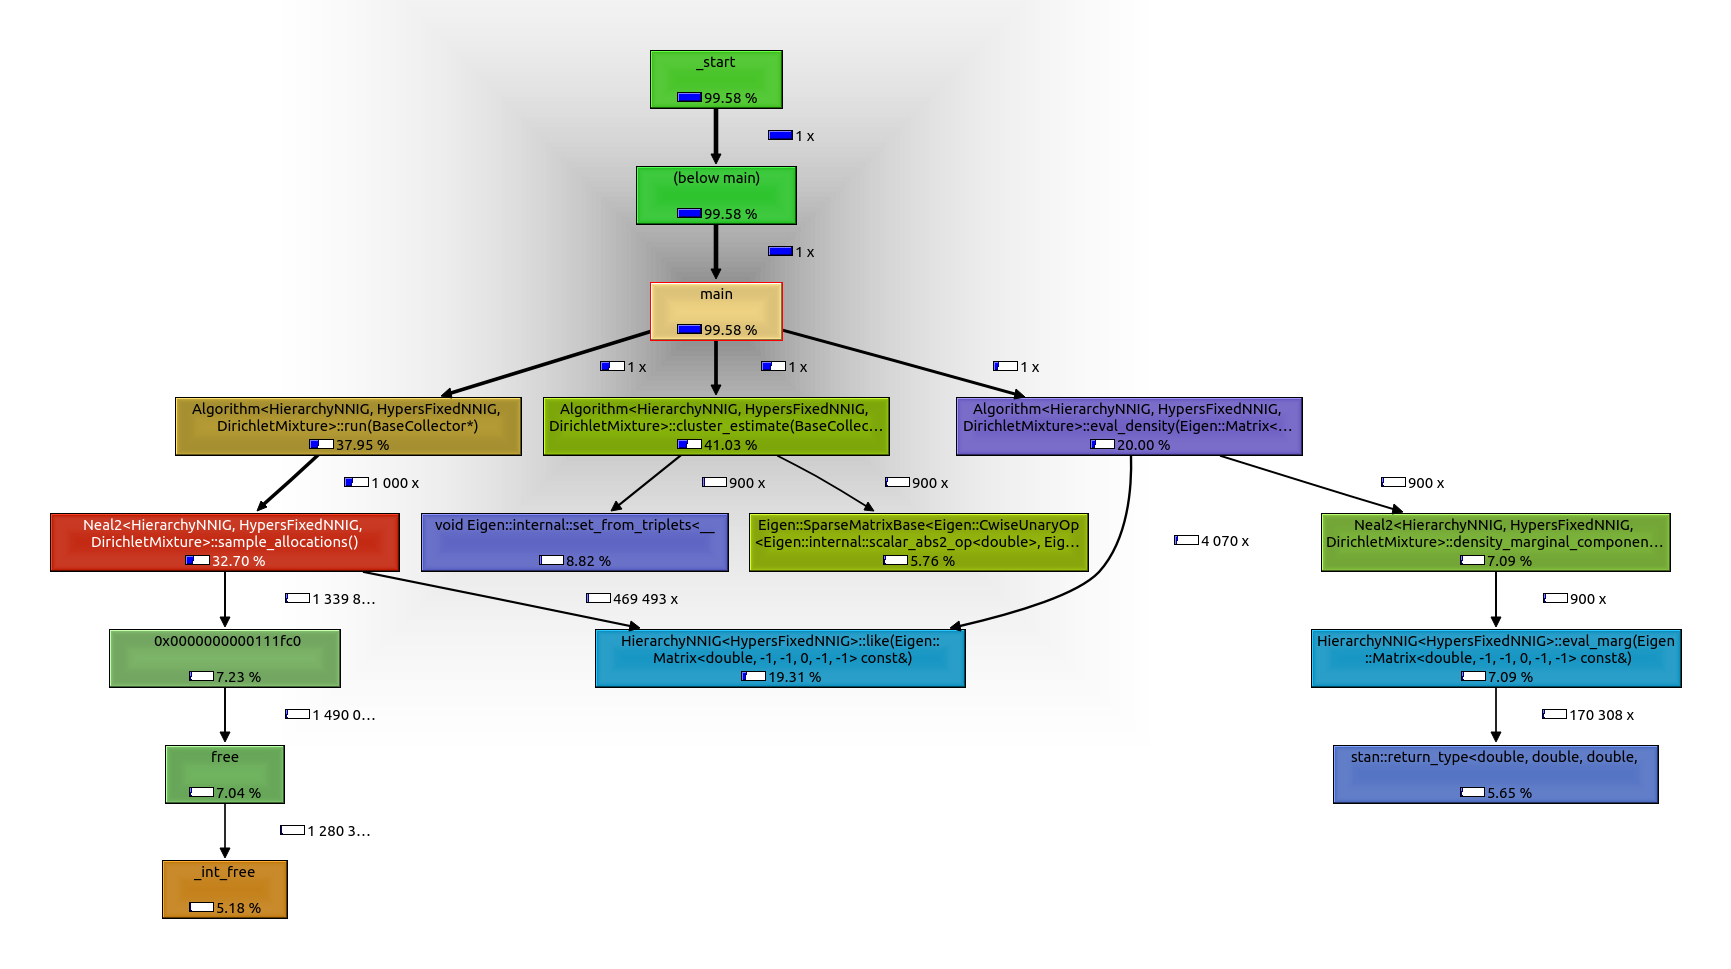
\includegraphics[scale=0.35]{etc/kcg_uni.png}
	%\captionsetup{labelformat=empty}
	%\caption{}
\end{figure}
The output of the univariate case produced the above dependence graph. %TODO check it is still above
The percentage inside the square is the proportion of the total time spent in that particular function across all calls to it.
The number followed by x tells instead the number of times that function was called. \\
We are first interested in the partitioning of the computation time between the different methods.
We note that \verb|run()| has slightly less than 40\% of the total time, while \verb|eval_density()| has around 20\%, and \verb|cluster_estimate()| slightly more than 40\%.
As for the lower-level operations in \verb|run()|, almost all the time is spent in \verb|step()|, more specifically in \verb|sample_allocations()| (33\%).
This also means that the cost of collecting the states into the \verb|MemoryCollector| is irrelevant.
Moreover, \verb|like()| is the most significant low-level utility function in the library, taking a total of 20\% of the total time across both \verb|run()| and \verb|eval_density()|. \\

Let us now compare these results with the multivariate case, as shown in the next page. %TODO check it still is in the next page
As for the general composition, \verb|run()| has now become less than 10\% of the total, with \verb|sample_allocations()| taking roughly half of that amount, while the \verb|eval_density()| part reaches almost 90\%.
This is to be expected since nearly all of the time is spent likelihood and marginal computation, which is much harder in 2D than in the univariate case due to the introduction of matrix algebra.
We can also note that as a side effect of the growth of the density estimation part, the percentage of time spent in \verb|cluster_estimate()| is now irrelevant, which makes sense since the computational costs of building a dissimilarity matrix is almost identical in all dimensions.
The most costly part of the density estimation is the unoptimized \verb|eval_marg()| (more than 60\%), presumably due to the presence of matrix inversions and Student's t evaluations, both of which require expensive Cholesky decompositions.
\begin{figure}[h]
	\hspace{-60pt}
	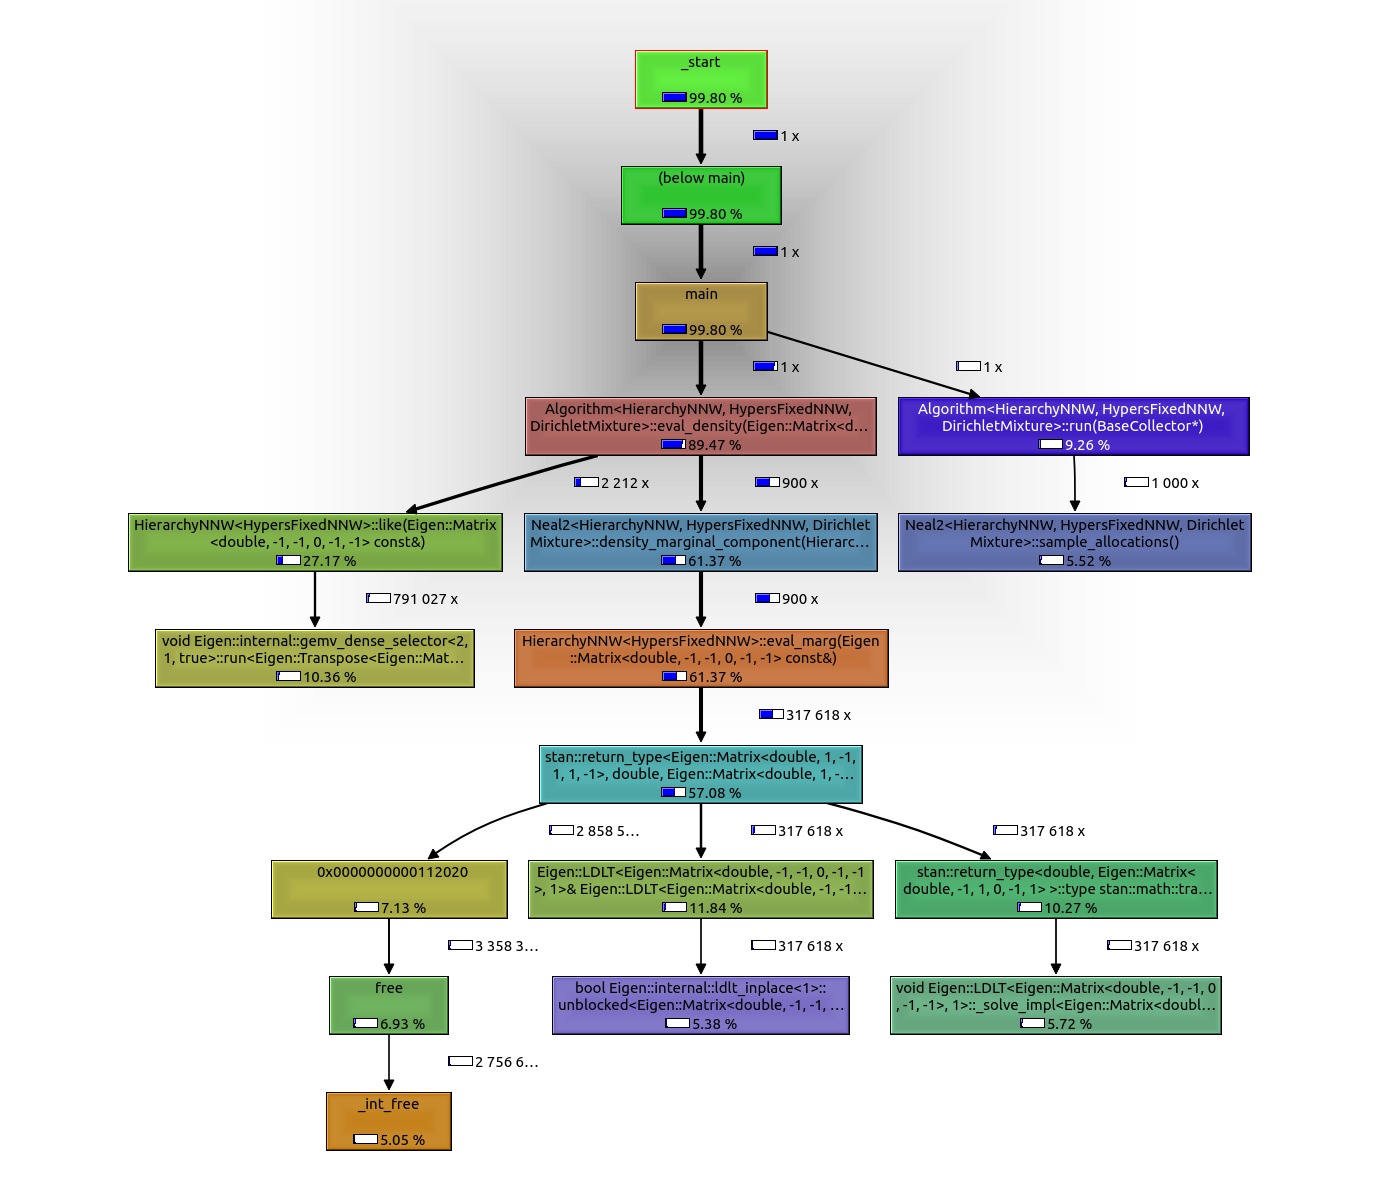
\includegraphics[scale=0.45]{etc/kcg_multi.png}
	%\captionsetup{labelformat=empty}
	%\caption{}
\end{figure}
On the contrary, we note that the usage of \verb|like()| is in the same order of magnitude as before (27\%).
Since the estimate algorithm is the same as before, this means that \verb|like()| is optimized enough for it to withstand the jump to the multidimensional case better than the other functions. \\
As for a final comparison with the case lacking the compiler flags described in section (\ref{opt-flags}), the optimization mainly impacts the multivariate case, with \verb|run()| being the main recipient, going from a whopping 58\% to the already mentioned 10\%.
In the univariate case, everything evenly benefits from the speedup, with the only relevant difference being for \verb|like()| which goes from over 30\% to 20\%.


\section{Limits}
Despite the optimizations in the \verb|cluster_estimate()| function, the storing of a number of large matrices still requires a considerable amount of memory.
In general, the Protobuf structures also become overwhelmingly large if the data dimension increases.
For these reasons, we were not able to run the multivariate Python tests (see chapter \ref{chap-py-test}) in higher dimensions such as $d=10$ and $d=20$ on our machines. \\
Another problem related to large dimensions arises when trying to run the \verb|Neal8| algorithm with 5-dimensional data.
At one point, the computed covariance matrix in one of the functions of the hierarchy becomes not symmetric.
Since a covariance/precision matrix must be symmetric and the Stan library implements a check for this property when passing such matrices as arguments to the density functions, the execution stops.
This error is likely due to the fact that the more the dimension of a space increases, the more its points will be far apart from each other -- this is the so-called ``curse of dimensionality''.
Since variance is a form of distance, the huge gap between points leads to a covariance matrix with large entries; due to the increased order of magnitude of these numbers, the floating-point approximations which are normally too small to appear become significant.
The hierarchy state is actually a precision matrix, which is the inverse of covariance and therefore should have very small values, but the computation of some covariance matrices is still required at some points.


% Part 3
%\part{Results}

\chapter{Results}
\section{Sensitivity analysis}
TODO
This clustering analysis was conducted on $n=100$ observations, the former 50 of which were iid sampled from a $\Nc(4,1)$ and the latter from a $\Nc(7,1)$.
We chose the prior parameters for the Normal-NIG model (\ref{nnig}) as follows: $\mu_0 = 5, \lambda_0 = 1, \alpha_0 = 2, \beta_0 = 2$.
The \verb|Neal8| algorithm with $m=3$ auxiliary blocks was run for 20000 iterations, and the first 5000 were discarded as burn-in, for a total of $K=15000$ valid iterations.
We will keep these parameters values fixed unless explicitly stated. \\
The following test data were all saved to \verb|.csv| files and used for the realization of plots with the \verb|ggplot2| R package.

\subsection{Oscillations}
After running the algorithm as described above with total mass $M=0.25$, we find that the obtained clusterings and local density estimates are highly fluctuating over the iterations of the algorithm, as shown in figure \ref{fig:fluctuations}:
\begin{figure}[h]
	\centering
	\begin{minipage}{0.5\textwidth}
		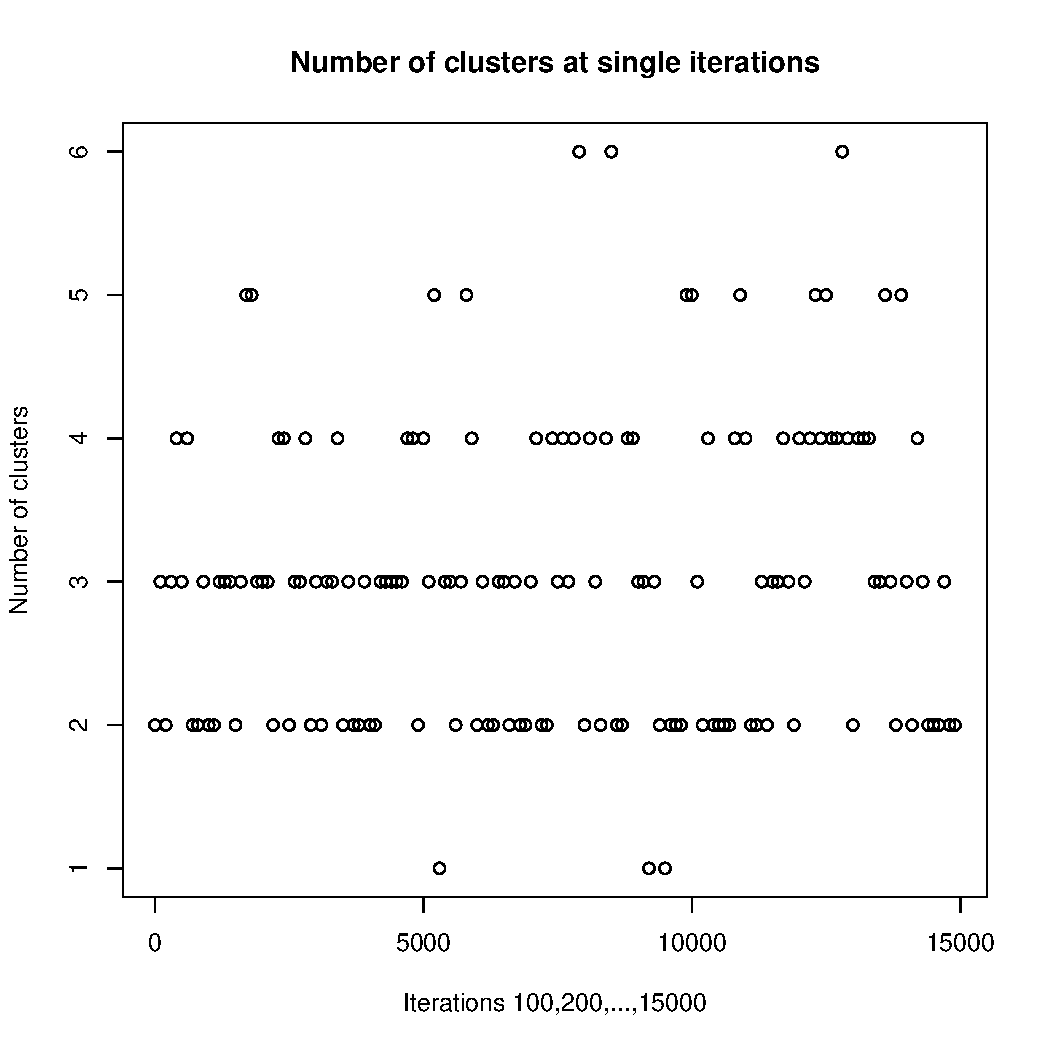
\includegraphics[scale=0.35]{etc/cardinalities_thinned.pdf}
	\end{minipage}%
	\begin{minipage}{0.5\textwidth}
		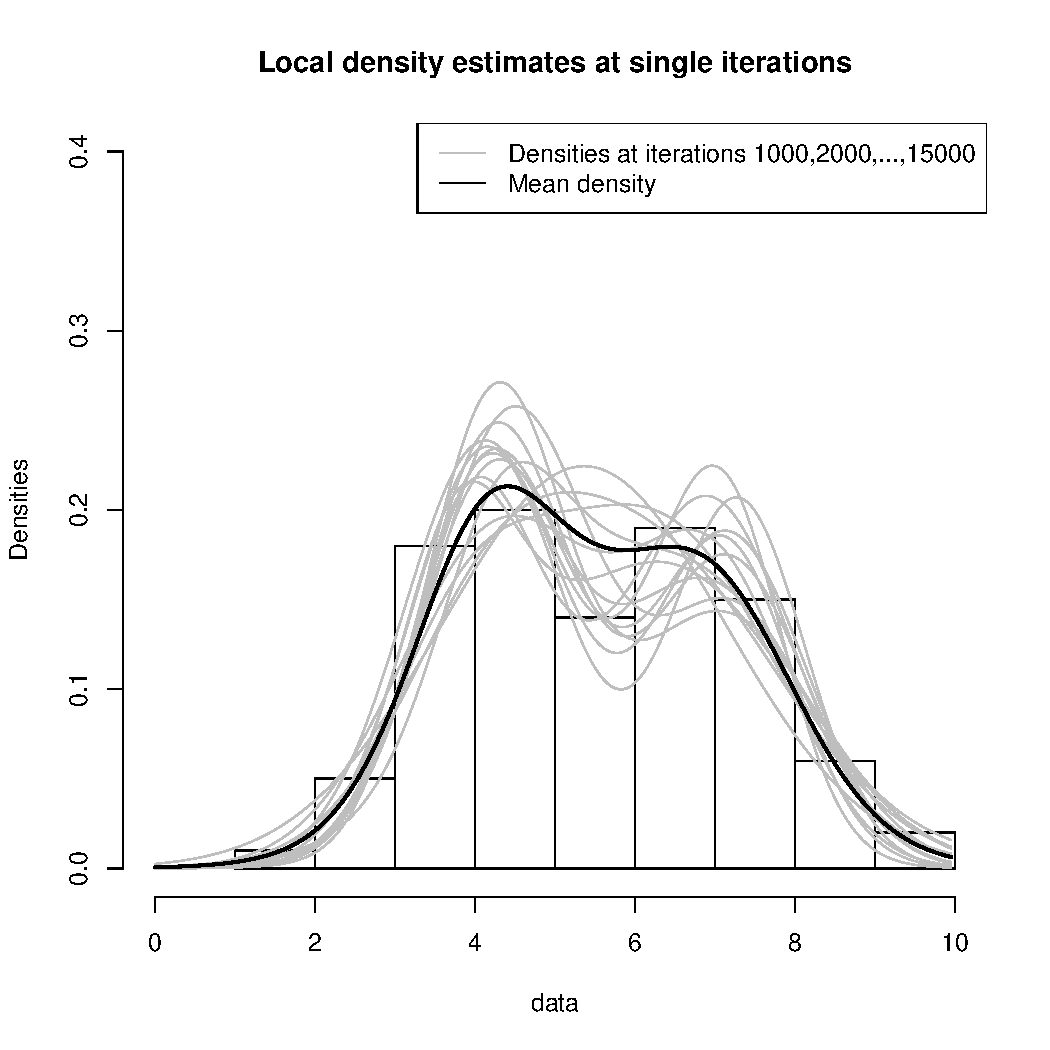
\includegraphics[scale=0.35]{etc/densities_iters.pdf}
	\end{minipage}
	\caption{Clustering and density fluctuations over iterations}

	\label{fig:fluctuations}

\end{figure}

In both plots, a thinning of one iteration every 100 and every 2500, respectively, was performed for better readability of the plot.
In the right side plot, the local densities are compared with the histogram of the data as well as the final estimate provided by the mean density.
We can see that the number of clusters at all iterations varies significantly between 1 and 6, even in the last thousands of iterations, and the same behavior applies to the local density estimates. 
This is further confirmation of the fact that the single iterations themselves do not converge.
Instead, as previously discussed, the convergence is in the \emph{mean}, both for the density estimate and for the average dissimilarity matrix which we use to find the best clustering.

\subsection{Total mass}
Let us now examine the role of the total mass parameter, $M$.
We ran the algorithm with several values for $M$ whilst keeping the other parameters unchanged from the ones indicated at the beginning of the section.
For each $M$, we saved the number of clusters of the best clustering produced by the algorithm, and studied the overall behavior varying $M$, shown in figure \ref{fig:n_clusters_M}.

\begin{figure}[h]
	\centering
	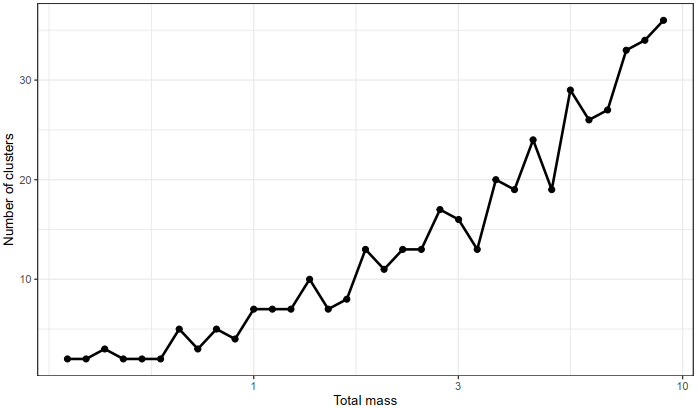
\includegraphics[scale=0.5]{etc/clusters.PNG}
	\caption{Number of clusters as a function of the total mass}

	\label{fig:n_clusters_M}

\end{figure}

Note that the values for $M$ were chosen so as to be evenly spaced in log-scale, thus the abscissa is in log-scale as well.
We can note that the clusters are increasing with the total mass.
This is consistent with the fact that the probability of creating a new cluster is proportional to $M$, as seen in (\ref{neal8prob}). \\
Moreover, we can see in figure \ref{fig:density_M} the density estimates for some of the values of $M$ (again, compared with the histogram of the data).

\clearpage

\begin{figure}[h]
	\centering
	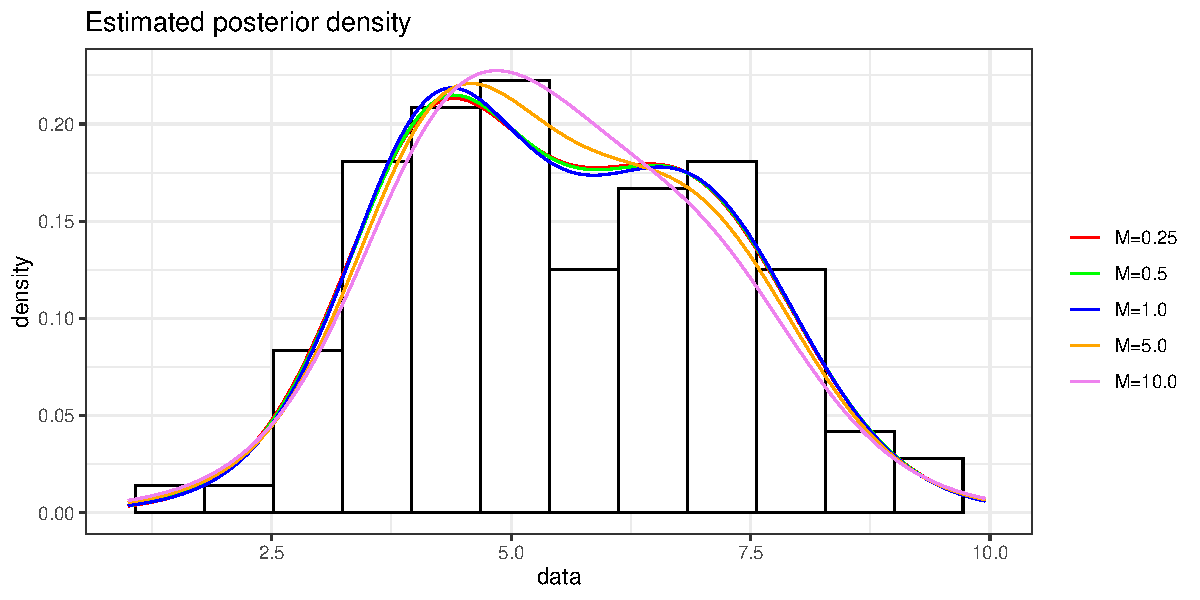
\includegraphics[scale=0.55]{etc/dens_withMm3.pdf}
	\caption{Density estimates varying the total mass}

	\label{fig:density_total_mass}
\end{figure}


In our case, lower values for the total mass account better for the distribution of the data points, with the modes being near the real expected values of the two normal distributions, 4 and 7.
On the other hand, higher values tend to clump together all 100 observations as though they were extracted from a single distribution.
As we can see, the total mass $M$ acts as smoothing parameter and, given its strong influence on the number of mixture components, it is a prime candidate for a prior distribution being put onto it.



\subsection{Auxiliary blocks}
We shall now try and change the number of auxiliary blocks $m$, and check how this impacts the density estimation.
For this test, a large total mass $M=10$ was chosen; the reason being that a small $M$ would not allow significant differences as $m$ changes.
Indeed, $m$ directly influences only the estimate (\ref{margneal8}) of the marginal distribution, that has a weight of $\frac{M}{M+n}$ (as seen in (\ref{localdens})), which is negligible if $M$ is small.
Therefore, $M=10$ was picked, and the result is displayed in figure \ref{fig:density_n_aux}.


\begin{figure}[h]
	\centering
	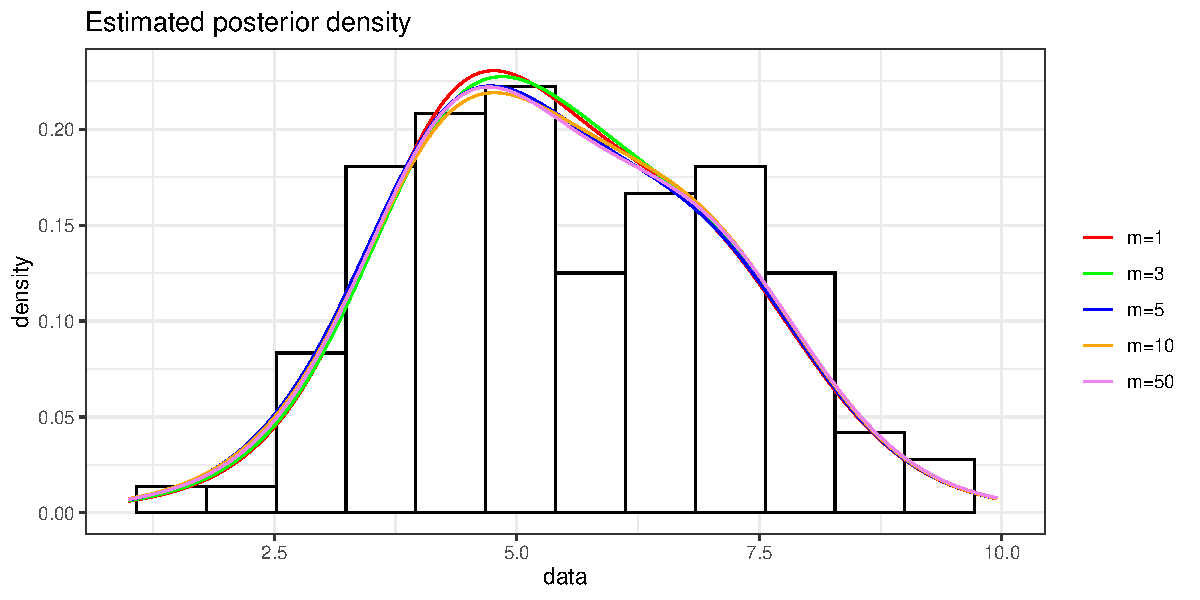
\includegraphics[scale=0.55]{etc/dens_withmM10.pdf}
	\caption{Density estimates varying the number of auxiliary blocks}

	\label{fig:density_n_aux}
\end{figure}

Note that a larger $m$ gives a better estimate of the marginal, because the sample mean is computed over a larger number of terms and the algorithm approximates the behavior of the algorithm \verb|Neal2|.



\subsection{Density components}
We now wish to visualize how the local density is computed at a given sample iteration.
Let us run again the \verb|Neal8| algorithm with both $M=0.25$ and $m=3$ fixed, and then use the \verb|cluster_estimate()| function to extract the best clustering for the data.
We find that it is at iteration 2490, which gives 2 clusters.
As shown in \ref{localdens}, each of these clusters has its own density estimate, which we refer to as \emph{component}, and a weight attached to it proportional to its cardinality.
The weighted sum of these components gives the ``full'' local estimate of the density for that iteration.
The plot in figure \ref{fig:components_density} shows both the \emph{weighted} components and their sum.
\begin{figure}[h]
	\centering
	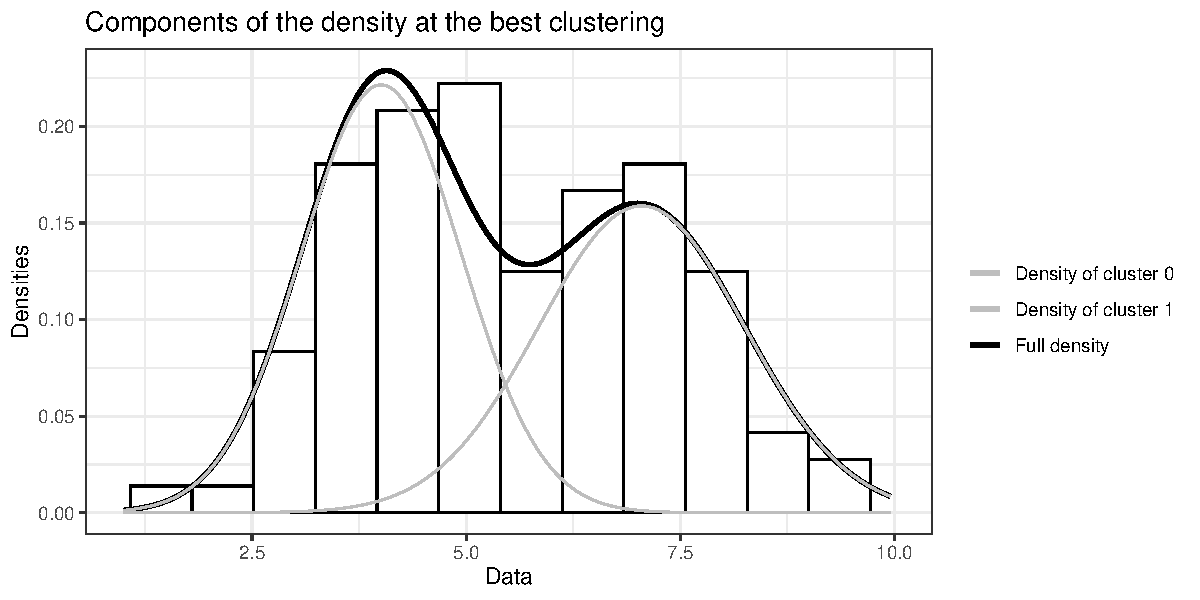
\includegraphics[scale=0.6]{etc/componentsM025m3_best.pdf}
	\caption{Weighted components and full density estimates}

	\label{fig:components_density}
\end{figure}

In this case the weights turn out to be approximately equal (0.52 and 0.48 respectively).
Again, the two components are concentrated around the true means (4 and 7) of the likelihoods of the data points, as expected. \\
In other cases, the best clustering may produce more than 2 clusters.
One such example is given by the best clustering of \verb|Neal8| run with $M=1$ (and $m=3$ as before), found at iteration 6611.
Although there are 7 clusters, all weights bar the first two are insignificant, as we can see in figure \ref{fig:cluster_weigths}, making the corresponding components have almost zero impact in the weighted sum of the local estimate.

\clearpage

\begin{figure}[h]
	\centering
	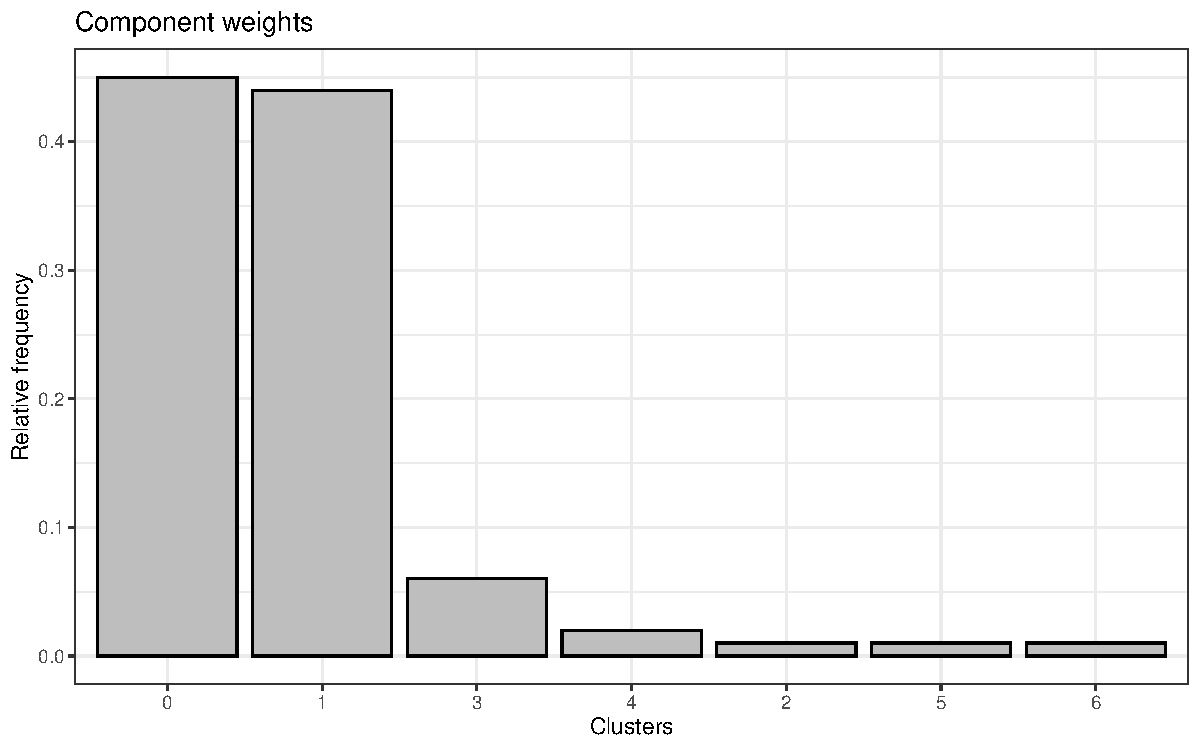
\includegraphics[scale=0.4]{etc/barplotM1m3.pdf}
	\caption{Clusters weights}

	\label{fig:cluster_weigths}
	
\end{figure}



\subsection{\texttt{Neal2} vs \texttt{Neal8}}
Finally, we ran the \verb|Neal2| algorithm with the same parameters as \verb|Neal8| (indicated at the beginning of the section) as well as $M=10$ for both.
Again, a rather large total mass was chosen in order to better highlight the difference in the marginal estimate.
In fact, in the \verb|Neal2| case, since the marginal distribution is known in closed form, the estimate is more accurate. A qualitative analysis is shown in figure \ref{fig:neal2_neal8}.

\begin{figure}[h]
	\centering
	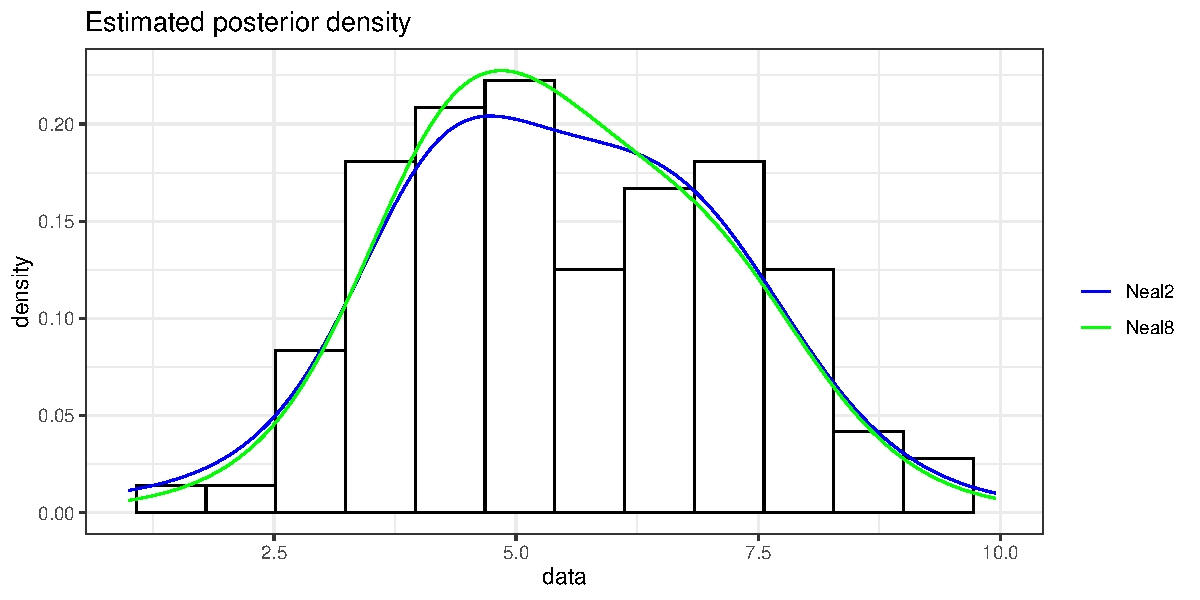
\includegraphics[scale=0.55]{etc/neal2_M10.pdf}
	\caption{Neal2 and Neal8 density estimates}

	\label{fig:neal2_neal8}
\end{figure}

\chapter{Python tests}
TODO \\
MAXITER 500, BURN-IN 100 \\
Univariati: \\
1) $y_i ~ 0.5 N(-3, 1) + 0.5 N(3, 1), i=1,... 200$ \\
$mu_0$ = 0.0 \\
lambda = 0.1 \\
a, b = 2 \\
Test 1: Rand index score: 1.0 \\
2) $y_i ~ 0.9 N(-5, 1) + 0.1 N(5, 1), i=1,... 1000$ \\
stessi parametri di prima \\
Test 2: Rand index score: 0.9879166470544726 \\
3) $y_i ~ 0.3 N(-2, 0.8^2) + 0.3 N(0, 0.8^2) + 0.4 N(2, 1) i=1,... 200$ \\
Test 3: Rand index score: 0.6656213747405262 \\
4) $y_i ~ 0.5 t(5, -5, 1 ) + 0.5 SkewNormal(2, -5, 1) i=1,... 400$ \\
Test 4: Rand index score: 0.9900498146844491 \\
Multivariati: \\
5) $y_i ~ 0.5 N((-3, -3), I) + 0.5 N((3, 3), I) i=1, ... 400$ \\
Test 5: Rand index score: 1.0 \\
6-8) dati come prima, all'aumentare della dimensione (d=5, 10, 20) \\
Test 6: Rand index score: 1.0

% TODO tutti i plot delle densità stimate e densità vere

\chapter{Extensions}
The \verb|bnplib| library has several possible extensions:
\begin{itemize}
	\item New types of \verb|Hypers| classes can be implemented, for example ones containing hyper-priors for some of the parameters if the model.
	The algorithm must be modified accordingly, for instance by implementing the currently empty extra step such as \verb|update_hypers()|.
	Changes depend on the type of parameter for which a prior is used; for example, a prior on the total mass parameter involves different steps than a prior on the parameters of the base measure.
	For a general outline of the necessary changes, see \cite{neal} section 7.
	\item Hierarchies other than the NNIG and NNW can be created.
	This is enough to run \verb|Neal8| and \verb|Neal2| by passing the class name as parameter, provided that the \verb|Hierarchy| class has the appropriate interface.
	\item The same goes for other mixtures and algorithm.
	A good starting point for the latter would be the blocked Gibbs algorithm, which would make use of the \verb|update_weights()| substep.
	\item Conjugacy-dependent algorithms such as \verb|Neal2| can be further re-adapted to account for non-conjugacy, for example by using an Hamiltonian Monte Carlo sampler.
	\item Code parallelization: in particular the \verb|cluster_estimate| function takes some time to compute the dissimilarity matrices.
	\item Finally, a \emph{full generalization} of the library might be possible.
	That is, given the distributions of the likelihood, hyperparameters, etc, one might want an algorithm that works for the chosen specific model without needing and explicit implementation for it.
	This means, among other things, that one has to handle non-conjugacy for the general case.
	The main issue is that Stan distribution functions do not accept vectors of parameter values as arguments; thus, the updated values for distributions must be explicitly enumerated and given as arguments one by one to the Stan function.
	This requires to know in advance the number of parameters for all such distributions, which is impossible in the general case.
	Some advanced C++ techniques may be used to circumvent this hindrance, such as argument unpackers that transform a vector into a list of function arguments, and variadic templates, which are templates that accept any number of arguments.
	Theoretically, the latter would also allow the use of priors on the parameters of the hyper-prior itself, and so on, adding layers of uncertainty ad libitum.
	Although it is a hard task, we do think it is possible to achieve with reasonable effort.
\end{itemize}


% Part 4
\part{Appendix}
\chapter{Distributions}
We include here all supports and probability density functions (p.d.f.) for the distributions mentioned in the report, in order of appearance:
\begin{itemize}
	\item Dirichlet distribution $\text{Dir}(\alpha_1, \dots, \alpha_k)$: a $k$-dimensional generalization of the Bernoulli distribution, given $\alpha_1,\dots,\alpha_k > 0$.
	It has support in the $k-1$-dimensional simplex.
	Its probability density function (p.d.f.) is
	$$f(\textbf x) = \frac{1}{B(\alpha_1, \dots, \alpha_k)} \prod_{i=1}^k x_i^{\alpha_i-1}$$
	with $B(\alpha_1, \dots, \alpha_k)$ being the $k$-dimensional Beta function that acts as a normalization constant.
	\item Gamma distribution $\text{Gamma}(\alpha,\beta)$: given $\alpha,\beta > 0$.
	It has support over all positive values, which is ideal for variances.
	Its p.d.f. is
	$$f(x) = \frac{\beta^\alpha}{\Gamma(\alpha)} x^{\alpha-1} \exp\{-\beta x\}$$
	with $\Gamma(\alpha)$ being the Euler-Gamma function.
	\item Wishart distribution $\text{Wish}(T_0, \nu)$: a $k$-dimensional generalization of the Gamma distribution.
	It has support over all matrices $X \in \RR^{k \times k}$ that are positive semi-definite.
	Its p.d.f. is
	$$f(X) = \frac{ (\det(X))^{(\nu-k-1)/2} \, \exp\{-\frac{1}{2} \text{tr}(T_0^{-1} X)\} }{ 2^{\nu k/2} \, (\det(X))^{\nu/2} \, \Gamma_k(\nu/2) } $$
	with $\Gamma_k(\alpha)$ being the $k$-dimensional Gamma function.
	\item Student's $t$ TODO (also others?)
\end{itemize}


\begin{thebibliography}{9}
	\bibitem{book} P. Muller, F. A. Quintana, \textit{Bayesian Nonparametric Data Analysis}
	
	\bibitem{neal} R. M. Neal (2000), \textit{Markov Chain Sampling Methods for Dirichlet Process Mixture Models}
	
	\bibitem{james} H. Ishwaran, L. F. James (2001), \textit{Gibbs Sampling Methods for Stick-Breaking Priors}
	
	\bibitem{integral} K. P. Murphy (2007), \textit{Conjugate Bayesian analysis of the Gaussian distribution}
	
	\bibitem{stan} Stan documentation: \url{http://mc-stan.org/math}. \\
	Code found at \url{https://github.com/stan-dev/math} (version 3.0.0 was used) and it also includes other needed libraries: Boost, Eigen, SUNDIALS, Intel TBB
	
	\bibitem{eigen} Eigen documentation: \url{https://eigen.tuxfamily.org/dox}. \\
	Code is included in the Stan package (version 3.3.3 is used there)
	
	\bibitem{proto} Protocol Buffers Tutorial for C++: \url{https://developers.google.com/protocol-buffers/docs/cpptutorial}. \\
	Code found at \url{https://github.com/protocolbuffers/protobuf} (version 3.11.0 was used)
	
	\bibitem{tutors} Codes of Mario Beraha and Riccardo Corradin for similar projects, found at \url{https://github.com/mberaha/partial_exchangeability} and \url{https://github.com/rcorradin/BNPmix} respectively
	
	\bibitem{beep} Course material for Bayesian Statistics: \url{https://beep.metid.polimi.it/web/2019-20-bayesian-statistics-alessandra-guglielmi-/}
\end{thebibliography}

\end{document}
